% I seguenti commenti speciali impostano:
% 1. 
% 2. PDFLaTeX come motore di composizione;
% 3. tesi.tex come documento principale;
% 4. il controllo ortografico italiano per l'editor.

% !TEX encoding = UTF-8
% !TEX TS-program = pdflatex
% !TEX root = tesi.tex
% !TEX spellcheck = it-IT

\documentclass[10pt,                    % corpo del font principale
               a4paper,                 % carta A4
               twoside,                 % impagina per fronte-retro
               openright,               % inizio capitoli a destra
               english,                 
               italian,                 
               ]{book}    

\usepackage[utf8]{inputenc}             % codifica di input; anche [latin1] va bene
                                        % NOTA BENE! va accordata con le preferenze dell'editor

%**************************************************************
% Importazione package
%************************************************************** 

%\usepackage{amsmath,amssymb,amsthm}    % matematica

\usepackage[english, italian]{babel}    % per scrivere in italiano e in inglese;
                                        % l'ultima lingua (l'italiano) risulta predefinita

\usepackage{bookmark}                   % segnalibri

\usepackage{caption}                    % didascalie

\usepackage{chngpage,calc}              % centra il frontespizio

\usepackage{csquotes}                   % gestisce automaticamente i caratteri (")

\usepackage{emptypage}                  % pagine vuote senza testatina e piede di pagina

\usepackage{epigraph}					% per epigrafi

\usepackage{eurosym}                    % simbolo dell'euro

\usepackage[T1]{fontenc}                % codifica dei font:
                                        % NOTA BENE! richiede una distribuzione *completa* di LaTeX

%\usepackage{indentfirst}               % rientra il primo paragrafo di ogni sezione

\usepackage{graphicx}                   % immagini

\usepackage{hyperref}                   % collegamenti ipertestuali



\usepackage[binding=5mm]{layaureo}      % margini ottimizzati per l'A4; rilegatura di 5 mm

\usepackage{listings}                   % codici

\usepackage{microtype}                  % microtipografia

\usepackage{mparhack,fixltx2e,relsize}  % finezze tipografiche

\usepackage{nameref}                    % visualizza nome dei riferimenti                                      

\usepackage[font=small]{quoting}        % citazioni

\usepackage{subfig}                     % sottofigure, sottotabelle

\usepackage[italian]{varioref}          % riferimenti completi della pagina

\usepackage[dvipsnames]{xcolor}         % colori

\usepackage{booktabs}                   % tabelle                                       
\usepackage{tabularx}                   % tabelle di larghezza prefissata                                    
\usepackage{longtable}                  % tabelle su più pagine                                        
\usepackage{ltxtable}                   % tabelle su più pagine e adattabili in larghezza

\usepackage[toc, acronym]{glossaries}   % glossario
                                        % per includerlo nel documento bisogna:
                                        % 1. compilare una prima volta tesi.tex;
                                        % 2. eseguire: makeindex -s tesi.ist -t tesi.glg -o tesi.gls tesi.glo
                                        % 3. eseguire: makeindex -s tesi.ist -t tesi.alg -o tesi.acr tesi.acn
                                        % 4. compilare due volte tesi.tex.

\usepackage[backend=biber,style=verbose-ibid,hyperref,backref]{biblatex}
                                        % eccellente pacchetto per la bibliografia; 
                                        % produce uno stile di citazione autore-anno; 
                                        % lo stile "numeric-comp" produce riferimenti numerici
                                        % per includerlo nel documento bisogna:
                                        % 1. compilare una prima volta tesi.tex;
                                        % 2. eseguire: biber tesi
                                        % 3. compilare ancora tesi.tex.

%**************************************************************
% file contenente le impostazioni della tesi
%**************************************************************

%**************************************************************
% Frontespizio
%**************************************************************
\newcommand{\myName}{Alberto Andeliero }                         % autore
\newcommand{\myTitle}{Recommendation system}                    
\newcommand{\myDegree}{Tesi di laurea triennale}                % tipo di tesi
\newcommand{\myUni}{Università degli Studi di Padova}           % università
\newcommand{\myFaculty}{Corso di Laurea in Informatica}         % facoltà
\newcommand{\myDepartment}{Dipartimento di Matematica}          % dipartimento
\newcommand{\myProf}{Tullio Vardanega }                          % relatore
\newcommand{\myLocation}{Padova}                                % dove
\newcommand{\myAA}{2015-2016}                                   % anno accademico
\newcommand{\myTime}{Apr 2016}                                  % quando


%**************************************************************
% Impostazioni di impaginazione
% see: http://wwwcdf.pd.infn.it/AppuntiLinux/a2547.htm
%**************************************************************

\setlength{\parindent}{14pt}   % larghezza rientro della prima riga
\setlength{\parskip}{0pt}   % distanza tra i paragrafi


%**************************************************************
% Impostazioni di biblatex
%**************************************************************
\bibliography{bibliografia} % database di biblatex 

\defbibheading{bibliography}
{
    \cleardoublepage
    \phantomsection 
    \addcontentsline{toc}{chapter}{\bibname}
    \chapter*{\bibname\markboth{\bibname}{\bibname}}
}

\setlength\bibitemsep{1.5\itemsep} % spazio tra entry

\DeclareBibliographyCategory{opere}
\DeclareBibliographyCategory{web}

\addtocategory{opere}{womak:lean-thinking}
\addtocategory{web}{site:agile-manifesto}

\defbibheading{opere}{\section*{Riferimenti bibliografici}}
\defbibheading{web}{\section*{Siti Web consultati}}


%**************************************************************
% Impostazioni di caption
%**************************************************************
\captionsetup{
    tableposition=top,
    figureposition=bottom,
    font=small,
    format=hang,
    labelfont=bf
}

%**************************************************************
% Impostazioni di glossaries
%**************************************************************

%**************************************************************
% Acronimi
%**************************************************************
\renewcommand{\acronymname}{Acronimi e abbreviazioni}

\newacronym[description={\glslink{umlg}{Unified Modeling Language}}]
    {uml}{UML}{Unified Modeling Language}

\newacronym[description={\glslink{ictg}{Information Communication Technology}}]
		{ict}{ICT}{Information Communication Technology}

\newacronym[description={\glslink{cmsg}{Content Management System}}]
		{cms}{CMS}{Content Management System}

\newacronym[description={\glslink{mvcg}{Model View Controller}}]
    {mvc}{MVC}{Model View Controller}

\newacronym[description={\glslink{daog}{Data Access Object}}]
    {dao}{DAO}{Data Access Object}

\newacronym[description={\glslink{ideg}{Integrated Development Environment}}]
    {ide}{IDE}{Integrated Development Environment}


\newacronym[description={\glslink{apig}{Application Program Interface}}]
    {api}{API}{Application Program Interface}

\newacronym[description={\glslink{jsong}{Javascript Object Notation}}]
    {json}{JSON}{Javascript Object Notation}

\newacronym[description={\glslink{restg}{Representational State Transfer}}]
    {rest}{REST}{Representational State Transfer}


%**************************************************************
% Glossario
%**************************************************************
\renewcommand{\glossaryname}{Glossario}

\newglossaryentry{core business}
{
    name=\glslink{core business}{Core business},
    text=core business,
    sort=core business,
    description={Il core business è l'attività principale di un'azienda, ovvero la base su cui si basa il fatturato e il guadagno a fine esercizio}
}

\newglossaryentry{ictg}
{
		name=\glslink{ict}{ICT},
		text=Information Communication Technology,
		sort=ict,
		description={sono l'insieme dei metodi e delle tecnologie che realizzano i sistemi di trasmissione, ricezione ed elaborazione di informazioni (tecnologie digitali comprese)}
}

\newglossaryentry{cmsg}
{
    name=\glslink{cms}{CMS},
    text=Content Management System,
    sort=content management system,
    description={strumento software installato su un server web studiato per facilitare la
gestione dei contenuti dei siti web, svincolando l’amministratore da conoscenze
tecniche di programmazione}
}

\newglossaryentry{mvcg}
{
    name=\glslink{mvc}{MVC},
    text=Model View Controller,
    sort=model view controller,
    description={il Model-View-Controller, in informatica, è un pattern architetturale molto diffuso nello sviluppo di sistemi software, in particolare nell’ambito della programmazione orientata agli oggetti, in grado di separare la logica di presentazione dei dati dalla logica di business}
}

\newglossaryentry{framework}
{
    name=\glslink{framework}{Framework},
    text=framework,
    sort=framework,
    description={in informatica, e specificatamente nello sviluppo software, un framework è un’architettura logica di supporto su cui un software può essere progettato e realizzato, spesso facilitandone lo sviluppo da parte del programmatore}
}

\newglossaryentry{daog}
{
    name=\glslink{dao}{DAO},
    text=Data Access Object,
    sort=data access object,
    description={è un pattern architetturale per la gestione della persistenza: si tratta fondamentalmente di una classe con relativi metodi che rappresenta un’entità tabellare di un RDBMS, usata principalmente in applicazioni web, per stratificare e isolare l’accesso ad una tabella/record tramite query (poste all’interno dei metodi della classe) ovvero al data layer da parte della business logic creando un maggiore livello di astrazione ed una più facile manutenibilità. I metodi del DAO con le rispettive query dentro verranno così richiamati dalle classi della business logic}
}

\newglossaryentry{ideg}
{
    name=\glslink{ide}{IDE},
    text=Integrated Development Environment,
    sort=Integrated Development Environment,
    description={software che fornisce allo sviluppatore numerosi aiuti durante lo sviluppo del codice. Esempi di aiuti sono la segnalazione degli errori di sintassi, interazione con strumenti di debug, suggerimenti di completamento del codice e strumenti per le build automatiche}
}

\newglossaryentry{apig}
{
    name=\glslink{api}{API},
    text=Application Program Interface,
    sort=api,
    description={in informatica con il termine \emph{Application Programming Interface API} (ing. interfaccia di programmazione di un'applicazione) si indica ogni insieme di procedure disponibili al programmatore, di solito raggruppate a formare un set di strumenti specifici per l'espletamento di un determinato compito all'interno di un certo programma. La finalità è ottenere un'astrazione, di solito tra l'hardware e il programmatore o tra software a basso e quello ad alto livello semplificando così il lavoro di programmazione}
}

\newglossaryentry{umlg}
{
    name=\glslink{uml}{UML},
    text=Unified Modeling Language,
    sort=uml,
    description={in ingegneria del software UML, Unified Modeling Language è un linguaggio di modellazione e specifica basato sul paradigma object-oriented. L'UML svolge un’importantissima funzione di "lingua franca" nella comunità della progettazione e programmazione a oggetti. Gran parte della letteratura di settore usa tale linguaggio per descrivere soluzioni analitiche e progettuali in modo sintetico e comprensibile a un vasto pubblico}
}

\newglossaryentry{jsong}
{
    name=\glslink{json}{JSON},
    text=Javascript Object Notation,
    sort=json,
    description={formato adatto per lo scambio dei dati in applicazioni client-server. Presenta una struttura semplice e di facile comprensione per l’uomo. Tale caratteristica ha contribuito alla sua rapida diffusione.}
}

\newglossaryentry{restg}
{
    name=\glslink{rest}{REST},
    text=Representational State Transfer,
    sort=rest,
    description={un tipo di architettura software per i sistemi di ipertesto distribuiti come il World Wide Web}
}
 % database di termini
\makeglossaries


%**************************************************************
% Impostazioni di graphicx
%**************************************************************
\graphicspath{{immagini/}} % cartella dove sono riposte le immagini


%**************************************************************
% Impostazioni di hyperref
%**************************************************************
\hypersetup{
    %hyperfootnotes=false,
    %pdfpagelabels,
    %draft,	% = elimina tutti i link (utile per stampe in bianco e nero)
    colorlinks=true,
    linktocpage=true,
    pdfstartpage=1,
    pdfstartview=FitV,
    % decommenta la riga seguente per avere link in nero (per esempio per la stampa in bianco e nero)
    %colorlinks=false, linktocpage=false, pdfborder={0 0 0}, pdfstartpage=1, pdfstartview=FitV,
    breaklinks=true,
    pdfpagemode=UseNone,
    pageanchor=true,
    pdfpagemode=UseOutlines,
    plainpages=false,
    bookmarksnumbered,
    bookmarksopen=true,
    bookmarksopenlevel=1,
    hypertexnames=true,
    pdfhighlight=/O,
    %nesting=true,
    %frenchlinks,
    urlcolor=webbrown,
    linkcolor=RoyalBlue,
    citecolor=webgreen,
    %pagecolor=RoyalBlue,
    %urlcolor=Black, linkcolor=Black, citecolor=Black, %pagecolor=Black,
    pdftitle={\myTitle},
    pdfauthor={\textcopyright\ \myName, \myUni, \myFaculty},
    pdfsubject={},
    pdfkeywords={},
    pdfcreator={pdfLaTeX},
    pdfproducer={LaTeX}
}

%**************************************************************
% Impostazioni di itemize
%**************************************************************
%\renewcommand{\labelitemi}{$\ast$}

%\renewcommand{\labelitemi}{$\bullet$}
%\renewcommand{\labelitemii}{$\cdot$}
%\renewcommand{\labelitemiii}{$\diamond$}
%\renewcommand{\labelitemiv}{$\ast$}


%**************************************************************
% Impostazioni di listings
%**************************************************************
\lstset{
    language=[LaTeX]Tex,%C++,
    keywordstyle=\color{RoyalBlue}, %\bfseries,
    basicstyle=\small\ttfamily,
    %identifierstyle=\color{NavyBlue},
    commentstyle=\color{Green}\ttfamily,
    stringstyle=\rmfamily,
    numbers=none, %left,%
    numberstyle=\scriptsize, %\tiny
    stepnumber=5,
    numbersep=8pt,
    showstringspaces=false,
    breaklines=true,
    frameround=ftff,
    frame=single
} 


%**************************************************************
% Impostazioni di xcolor
%**************************************************************
\definecolor{webgreen}{rgb}{0,.5,0}
\definecolor{webbrown}{rgb}{.6,0,0}


%**************************************************************
% Altro
%**************************************************************

\newcommand{\omissis}{[\dots\negthinspace]} % produce [...]

% eccezioni all'algoritmo di sillabazione
\hyphenation
{
    ma-cro-istru-zio-ne
    gi-ral-din
}

\newcommand{\sectionname}{sezione}
\addto\captionsitalian{\renewcommand{\figurename}{figura}
                       \renewcommand{\tablename}{tabella}}

\newcommand{\glsfirstoccur}{\ap{{[g]}}}

\newcommand{\intro}[1]{\emph{\textsf{#1}}}

%**************************************************************
% Environment per ``rischi''
%**************************************************************
\newcounter{riskcounter}                % define a counter
\setcounter{riskcounter}{0}             % set the counter to some initial value

%%%% Parameters
% #1: Title
\newenvironment{risk}[1]{
    \refstepcounter{riskcounter}        % increment counter
    \par \noindent                      % start new paragraph
    \textbf{\arabic{riskcounter}. #1}   % display the title before the 
                                        % content of the environment is displayed 
}{
    \par\medskip
}

\newcommand{\riskname}{Rischio}

\newcommand{\riskdescription}[1]{\textbf{\\Descrizione:} #1.}

\newcommand{\risksolution}[1]{\textbf{\\Soluzione:} #1.}

%**************************************************************
% Environment per ``use case''
%**************************************************************
\newcounter{usecasecounter}             % define a counter
\setcounter{usecasecounter}{0}          % set the counter to some initial value

%%%% Parameters
% #1: ID
% #2: Nome
\newenvironment{usecase}[2]{
    \renewcommand{\theusecasecounter}{\usecasename #1}  % this is where the display of 
                                                        % the counter is overwritten/modified
    \refstepcounter{usecasecounter}             % increment counter
    \vspace{10pt}
    \par \noindent                              % start new paragraph
    {\large \textbf{\usecasename #1: #2}}       % display the title before the 
                                                % content of the environment is displayed 
    \medskip
}{
    \medskip
}

\newcommand{\usecasename}{UC}

\newcommand{\usecaseactors}[1]{\textbf{\\Attori Principali:} #1. \vspace{4pt}}
\newcommand{\usecasepre}[1]{\textbf{\\Precondizioni:} #1. \vspace{4pt}}
\newcommand{\usecasedesc}[1]{\textbf{\\Descrizione:} #1. \vspace{4pt}}
\newcommand{\usecasepost}[1]{\textbf{\\Postcondizioni:} #1. \vspace{4pt}}
\newcommand{\usecasealt}[1]{\textbf{\\Scenario Alternativo:} #1. \vspace{4pt}}

%**************************************************************
% Environment per ``namespace description''
%**************************************************************

\newenvironment{namespacedesc}{
    \vspace{10pt}
    \par \noindent                              % start new paragraph
    \begin{description} 
}{
    \end{description}
    \medskip
}

\newcommand{\classdesc}[2]{\item[\textbf{#1:}] #2}


\colorlet{punct}{red!60!black}
\definecolor{background}{HTML}{EEEEEE}
\definecolor{delim}{RGB}{20,105,176}
\colorlet{numb}{magenta!60!black}
\lstdefinelanguage{json}{
    basicstyle=\normalfont\ttfamily\scriptsize,
    numbers=left,
    numberstyle=\scriptsize,
    stepnumber=1,
    numbersep=6pt,
    showstringspaces=false,
    breaklines=true,
    frame=lines,
    backgroundcolor=\color{background},
    literate=
     *{0}{{{\color{numb}0}}}{1}
      {1}{{{\color{numb}1}}}{1}
      {2}{{{\color{numb}2}}}{1}
      {3}{{{\color{numb}3}}}{1}
      {4}{{{\color{numb}4}}}{1}
      {5}{{{\color{numb}5}}}{1}
      {6}{{{\color{numb}6}}}{1}
      {7}{{{\color{numb}7}}}{1}
      {8}{{{\color{numb}8}}}{1}
      {9}{{{\color{numb}9}}}{1}
      {:}{{{\color{punct}{:}}}}{1}
      {,}{{{\color{punct}{,}}}}{1}
      {\{}{{{\color{delim}{\{}}}}{1}
      {\}}{{{\color{delim}{\}}}}}{1}
      {[}{{{\color{delim}{[}}}}{1}
      {]}{{{\color{delim}{]}}}}{1},
}                     % file con le impostazioni personali

\begin{document}
%**************************************************************
% Materiale iniziale
%**************************************************************
\frontmatter
% !TEX encoding = UTF-8
% !TEX TS-program = pdflatex
% !TEX root = ../tesi.tex
% !TEX spellcheck = it-IT

%**************************************************************
% Frontespizio 
%**************************************************************
\begin{titlepage}

\begin{center}

\begin{LARGE}
\textbf{\myUni}\\
\end{LARGE}

\vspace{10pt}

\begin{Large}
\textsc{\myDepartment}\\
\end{Large}

\vspace{10pt}

\begin{large}
\textsc{\myFaculty}\\
\end{large}

\vspace{30pt}
\begin{figure}[htbp]
\begin{center}

\includegraphics[height=6cm]{logo-unipd}
\end{center}
\end{figure}
\vspace{30pt} 

\begin{LARGE}
\begin{center}
\textbf{\myTitle}\\
\end{center}
\end{LARGE}

\vspace{10pt} 

\begin{large}
\textsl{\myDegree}\\
\end{large}

\vspace{40pt} 

\begin{large}
\begin{flushleft}
\textit{Relatore}\\ 
\vspace{5pt} 
Prof. \myProf
\end{flushleft}

\vspace{0pt} 

\begin{flushright}
\textit{Laureando}\\ 
\vspace{5pt} 
\myName
\end{flushright}
\end{large}

\vspace{40pt}

\line(1, 0){338} \\
\begin{normalsize}
\textsc{Anno Accademico \myAA}
\end{normalsize}

\end{center}
\end{titlepage} 
% !TEX encoding = UTF-8
% !TEX TS-program = pdflatex
% !TEX root = ../tesi.tex
% !TEX spellcheck = it-IT

%**************************************************************
% Colophon
%**************************************************************
\clearpage
\phantomsection
\thispagestyle{empty}

\hfill

\vfill

\noindent\myName: \textit{\myTitle,}
\myDegree,
\textcopyright\ \myTime.
% !TEX encoding = UTF-8
% !TEX TS-program = pdflatex
% !TEX root = ../tesi.tex
% !TEX spellcheck = it-IT

%**************************************************************
% Dedica
%**************************************************************
\cleardoublepage
\phantomsection
\thispagestyle{empty}
\pdfbookmark{Dedica}{Dedica}

\vspace*{3cm}



\medskip

\begin{center}
alla mia famiglia
\end{center}

% !TEX encoding = UTF-8
% !TEX TS-program = pdflatex
% !TEX root = ../tesi.tex
% !TEX spellcheck = it-IT

%**************************************************************
% Sommario
%**************************************************************
\cleardoublepage
\phantomsection
\pdfbookmark{Sommario}{Sommario}
\begingroup
\let\clearpage\relax
\let\cleardoublepage\relax
\let\cleardoublepage\relax

\chapter*{Sommario}

Il presente documento descrive il lavoro svolto durante il periodo di stage, della durata di circa trecento ore, dal laureando \myName presso l'azienda Nextep S.r.l. a Carmignano Di Brenta(PD).
%L'obbiettivo dello stage era quello di sviluppare un modulo software che permettesse di fornire una raccomandazione a seconda del comportamento dell'utente,
%\vfill
%
%\selectlanguage{english}
%\pdfbookmark{Abstract}{Abstract}
%\chapter*{Abstract}
%
%\selectlanguage{italian}

\endgroup			

\vfill


%% !TEX encoding = UTF-8
% !TEX TS-program = pdflatex
% !TEX root = ../tesi.tex
% !TEX spellcheck = it-IT

%**************************************************************
% Ringraziamenti
%**************************************************************
\cleardoublepage
\phantomsection
\pdfbookmark{Ringraziamenti}{ringraziamenti}

\begin{flushright}{
	\slshape    
	``Always code as if the guy who ends up maintaining your code will be a violent psychopath who knows where you live''} \\ 
	\medskip
    --- John Woods
\end{flushright}

\bigskip

\begingroup
\let\clearpage\relax
\let\cleardoublepage\relax
\let\cleardoublepage\relax

\chapter*{Ringraziamenti}

\noindent \textit{Vorrei ringraziare il Prof. Tullio Vardanega e mia sorella Irene, per il supporto fornitomi durante la stesura del lavoro.}\\
\bigskip

\noindent\textit{\myLocation, \myTime}
\hfill \myName

\endgroup

 da redigere
% !TEX encoding = UTF-8
% !TEX TS-program = pdflatex
% !TEX root = ../tesi.tex
% !TEX spellcheck = it-IT

%**************************************************************
% Indici
%**************************************************************
\cleardoublepage
\pdfbookmark{\contentsname}{tableofcontents}
\setcounter{tocdepth}{2}
\tableofcontents
%\markboth{\contentsname}{\contentsname} 
\clearpage

\begingroup 
    \let\clearpage\relax
    \let\cleardoublepage\relax
    \let\cleardoublepage\relax
    %*******************************************************
    % Elenco delle figure
    %*******************************************************    
    \phantomsection
    \pdfbookmark{\listfigurename}{lof}
    \listoffigures

    \vspace*{8ex}

    %*******************************************************
    % Elenco delle tabelle
    %*******************************************************
    \phantomsection
    \pdfbookmark{\listtablename}{lot}
    \listoftables
        
    \vspace*{8ex}
\endgroup

\cleardoublepage

\cleardoublepage

%**************************************************************
% Materiale principale
%**************************************************************
\mainmatter
% !TEX encoding = UTF-8
% !TEX TS-program = pdflatex
% !TEX root = ../tesi.tex
% !TEX spellcheck = it-IT

%**************************************************************
\chapter{L'azienda}
\label{cap:azienda}
%**************************************************************
\intro{Questo capitolo tratta dettagliatamente della azienda ospitante, il suo \emph{business}, l'organizzazione interna e l'innovazione.}\\




%***************************************************************************************
\section{Presentazione azienda}
Questa sezione descrive l'azienda che ha ospitato lo \emph{stage}, elencando generalità e la struttura generale dell'azienda. Inoltre si illustrano alcuni prodotti e i servizi offerti da Nextep srl, alla propria clientela.

\subsection{L'azienda}
L'azienda con cui ho svolto lo stage formativo è Nextep srl\footnote{\url{http://www.nextep.it/}}, la cui sede operativa si trova a Carmignano Di Brenta(PD). Nextep è una società fondata nel 2000 che opera nel settore dell'informatica e della comunicazione. Il \emph{\gls{core business}} dell'azienda, è riconosciuto nelle attività di progettazione, realizzazione e gestione di infrastrutture di \emph{Information and Digital Communication Technology}. L'organico di Nextep srl è formato da una ventina di persone, suddivise tra \emph{web marketing} e tecnici (sviluppatori, grafici e sistemisti). L'ambiente di lavoro è condiviso con altre due aziende: Allos  e Zero12. Allos si occupa della formazione del capitale umano di organizzazioni medio grandi, mentre Zero12  si occupa di servizi \emph{cloud} e applicazioni \emph{mobile}. Il risultato è un ambiente di \emph{co-working}, dove le competenze del singolo vengono messe a disposizione di tutti, in modo da facilitare la crescita professionale dei dipendenti delle varie aziende. Non è raro che le tre aziende collaborino tra di loro per la realizzazione di alcuni progetti.
\begin{figure}[h]
\centering

\includegraphics[scale=0.20]{immagini/logo_nextep}
\caption{Logo di Nextep srl}
\label{fig:logo_nextep}
\end{figure}

\subsection{Prodotti e servizi}
Il principale settore di attività dell'azienda è il \emph{Web}. Nextep è specialista nella progettazione e sviluppo di siti \emph{web}, portali, \emph{social intranet} e soluzioni di \emph{e-commerce}. L'azienda fornisce sistemi per il \emph{knowledge management}, che sono dei sistemi per raccogliere, sviluppare, conservare e rendere accessibile la conoscenza delle persone che fanno parte di una organizzazione. Si occupa inoltre dello sviluppo di  applicazioni mobile. L'azienda pone il suo focus, nella realizzazione di sistemi con interfacce innovative e soprattutto accessibili all'utente, grazie alle competenze acquisite nel ramo della \emph{User Interface} e \emph{User Experience}. Realizza sistemi per l'integrazione con tecnologie e servizi di \emph{Cloud Computing}.\\
%Nello specifico l'azienda si occupa di:
%\begin{itemize}
%\item Progettazione e sviluppo di siti web e portali;
%\item Progettazione e sviluppo di Social Intranet e capitalizzazione della cultura aziendale;
%\item Progettazione e sviluppo di soluzioni di e-commerce;
%\item Studio, Progettazione e Realizzazione di Applicazioni Mobile;
%\item Studio e Progettazione delle Grafica/User Experience (UX);
%\item Integrazione con tecnologie e servizi di Cloud Computing;
%\item Analisi e progettazione di ecosistemi per siti web, portali, social internet, infrastrutture IT.
%\item Analisi, Ideazione e Realizzazione di azioni di web marketing.
%\end{itemize}
I principali servizi offerti da Nextep srl ai propri clienti sono:
\begin{itemize}
\item Fornitura di servizi a canone (\emph{server virtuali}, applicazioni \emph{web}, servizi di \emph{monitoring} di infrastrutture \emph{\gls{ict}}, \emph{backup-online}, canoni di assistenza e manutenzione dei sistemi, canoni di gestione dei sistemi);
\item Elaborazione dati, analisi e supporto decisionale in ambito \emph{web marketing}, \emph{social marketing} e \emph{social intranet};
%\item Consulenza e formazione di web marketing, social marketing, web analytics;
\item Servizio Clienti, attività di supporto tecnico e di gestione di infrastrutture \emph{\gls{ict}} e siti \emph{web}.
\end{itemize}
\begin{figure}[h]
\centering
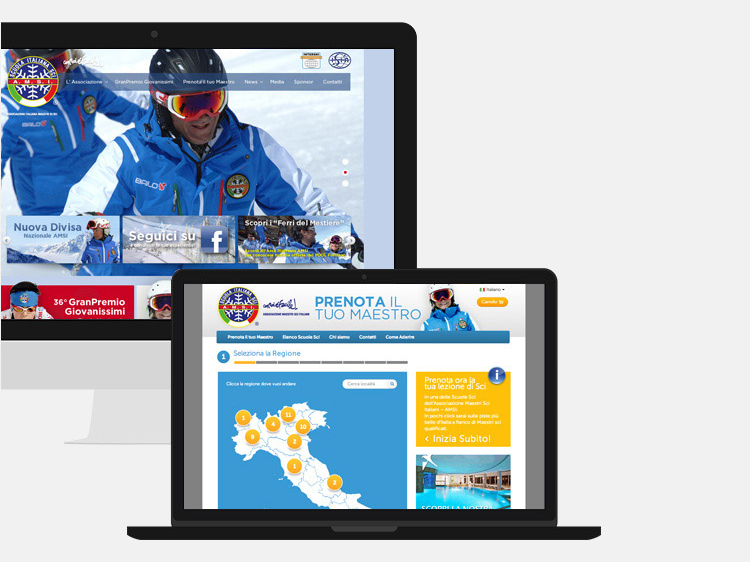
\includegraphics[scale=0.35]{immagini/amsi.jpg}
\caption{Sito Associazione Maestri Sci Italiani: realizzato da Nextep. Immagine tratta da \href{http://www.nextep.it/}{Nextep}}
\label{fig:amsi}
\end{figure}
In particolare l'azienda, fornisce servizi per migliorare l'efficacia delle strategie di comunicazione \emph{web}, dedicando particolare attenzione alla reputazione e all'identità digitale. Collabora, inoltre, assieme alle aziende nella gestione delle informazioni digitali, della sicurezza e della disponibilità dei dati e delle applicazioni. Infine nel ramo del \emph{marketing}, Nextep fornisce consulenza \emph{web marketing}, \emph{social marketing} e \emph{web analytics}.

\subsection{Tecnologie di riferimento}
Essendo il \emph{web} un settore soggetto a continue evoluzioni, le tecnologie utilizzate cambiano col tempo. Nextep cerca di aggiornare le tecnologie utilizzate, in modo da fornire ai propri clienti prodotti sempre migliori e innovativi.
\begin{figure}[h]
\centering
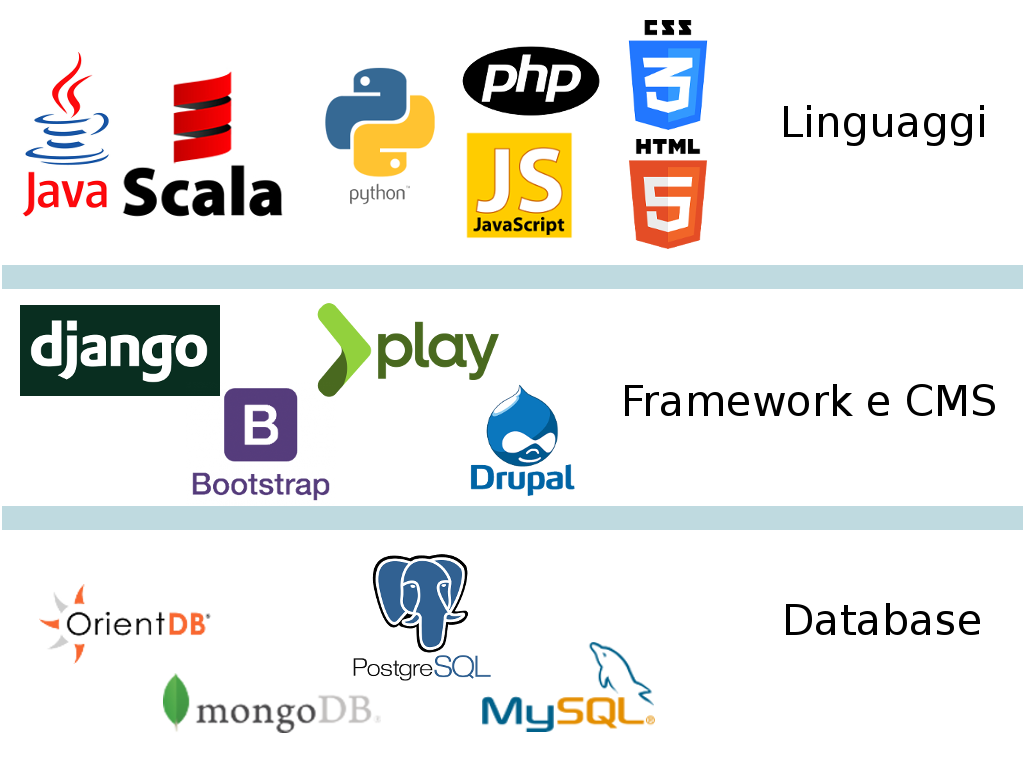
\includegraphics[scale=0.35]{immagini/tecnologie}
\caption{Classificazione delle tecnologie utilizzate}
\label{fig:tecnologie-utilizzate}
\end{figure}

\subsubsection{Linguaggi di programmazione}
L'azienda lavora principalmente in ambito \emph{web}, quindi utilizza i linguaggi di programmazione più moderni per lo sviluppo dei prodotti. I linguaggi di programmazione più utilizzati in ordine di importanza sono: Php, Python, Java e Scala. Per quanto riguarda le interfacce grafiche naturalmente utilizza tecnologie quali Html5, Css3 e Javascript.

\subsubsection{Framework e CMS}
\begin{description}
\item[Django] è un \emph{web \gls{framework} open source} per lo sviluppo di applicazioni \emph{web}, scritto in linguaggio Python, seguendo il \emph{pattern} \gls{mvc}. Fornisce nativamente delle applicazioni, per la gestione dei contenuti e degli accessi.
\item[Play Framework] è un \emph{web \gls{framework} open source} scritto in Java e Scala, che implementa il \emph{pattern} \gls{mvc}. Il suo scopo è di migliorare la produttività degli sviluppatori, usando il paradigma \emph{Convention Over Configuration}.\newpage
\item[Bootstrap] è \gls{framework} per la creazione di siti e applicazioni per il \emph{web}. Essa contiene modelli di progettazione basati su Html e Css. Necessarie per la tipografia, che per le varie componenti dell'interfaccia come moduli, bottoni e navigazione, e altri componenti dell'interfaccia.
\item[Drupal] è una piattaforma \emph{software} di \emph{\gls{cms}}, modulare, scritta in linguaggio Php e distribuita sotto licenza GNU GPL. Grazie alla sua architettura modulare, permette il riutilizzo sistematico del codice scritto e quindi un vantaggio, in termini di tempo e manutenzione.
\end{description}

\subsubsection{Database}
Il \emph{team} di sviluppo utilizza per la persistenza sia \emph{database} relazionali, sia non-relazionali.\\Fra i \emph{database} relazionali impiega per la maggiore le tecnologie quali MySql, Sql Server e PostgreSql. Per quanto riguarda i \emph{database} non-relazionali utilizza soluzioni come MongoDB oppure OrientDB. A seconda del contesto vengono studiati i pro e contro, in modo da poter trarre tutti i vantaggi possibili.
%***************************************************************************************




%***************************************************************************************
\newpage
\section{Processi aziendali}
Questa sezione illustra l'organizzazione interna dell'azienda, descritta per processi.
\begin{figure}[h]
\centering
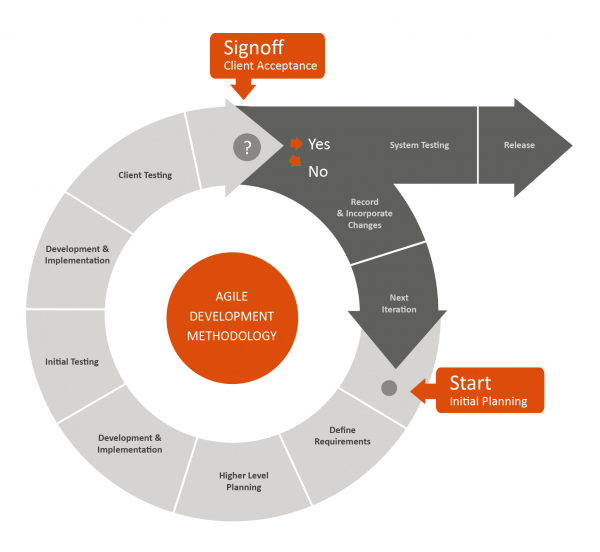
\includegraphics[scale=0.65]{immagini/agileo}
\caption{Diagramma della metodologia di sviluppo \emph{agile}. Immagine tratta da \href{http://blogs.globalteckz.com/characteristics-of-agile-methodology-in-software-development/}{GlobalTeckz}.}
\label{fig:agile}
\end{figure}
\subsection{Metodologia agile}
L'azienda per la gestione dei progetti adotta la metodologia \emph{agile}\footnote{\url{http://www.agilemanifesto.org/}}.\\Questa metodologia si basa su 4 principi:
\begin{itemize}
\item Gli individui e le interazioni più che i processi e gli strumenti;
\item Il \emph{software} funzionante più che la documentazione esaustiva;
\item La collaborazione col cliente più che la negoziazione dei contratti;
\item Rispondere al cambiamento più che seguire un piano.
\end{itemize}
In particolare tra le metodologie \emph{agile} l'azienda segue nello specifico il modello \emph{Scrum}, dove pianifica ciclicamente degli \emph{sprint}(un periodo di 2-4 settimane).
\newpage
Gli elementi costruttivi principali in \emph{Scrum} sono:
\begin{itemize}
\item \textbf{Product Backlog}, è un documento ad alto livello per l'intero progetto. Contiene una lista delle funzionalità desiderate, con priorità assegnate in base al valore di \emph{business} e  i \emph{Backlog Item} che sono descrizioni di tutte le caratteristiche richieste;
\item \textbf{Sprint Backlog}, è un documento che contiene informazioni su come il \emph{team} sta procedendo nell'implementare le funzionalità, per lo \emph{sprint} successivo. Le funzionalità vengono prelevate dalla pila del documento di \emph{Product Backlog}, in una quantità fattibile per essere realizzata nello \emph{sprint};
\item \textbf{Burn Down Chart}, è un grafico che rappresenta il lavoro nello \emph{Sprint Backlog} che deve essere ancora completato. Aggiornato ogni giorno, dà una semplice visione di come procede lo \emph{sprint};
\item \textbf{Incremento}, è la somma di tutti gli elementi del \emph{Product Backlog}, completati durante uno \emph{sprint} e tutti gli \emph{sprint} precedenti.
\end{itemize}
Le principali pratiche che Nextep svolge sono:
\begin{itemize}
\item \textbf{Daily scrum}, detto anche \emph{stand up}, è una riunione che tiene quotidianamente e serve per verificare lo stato di avanzamento durante uno \emph{sprint};
\item \textbf{Scrum of Scrums}, è una riunione che tiene meno frequentemente del \emph{Daily Scrum}. Consente ai \emph{team} di discutere del loro lavoro, concentrandosi su aree di sovrapposizione e d'integrazione;
\item \textbf{Sprint Planning Meeting}, è una riunione che l'azienda svolge all'inizio di ogni \emph{sprint}. Vengono pianificati gli obiettivi con relative priorità e le tempistiche. In questa riunione, partecipano \emph{Product Owner}, \emph{Scrum Master}, intero \emph{Scrum Team} e tutti i \emph{manager} del caso interessati o dai rappresentanti della clientela;
\item \textbf{Sprint Review}, al termine dello \emph{sprint} l'azienda svolge questa riunione per ispezionare l'incremento e adattare, se necessario, il \emph{Product Backlog}. In conformità a questo e dei cambiamenti al \emph{Product Backlog}, fatti durante lo \emph{sprint}, i partecipanti pianificano il prossimo incremento;
\item \textbf{Sprint Retrospective Meeting}, si svolge dopo la \emph{Sprint Review}, in questa occasione lo \emph{Scrum Team} ispeziona se stesso e crea un piano di miglioramento, da attuare durante il successivo \emph{sprint}.
\end{itemize}
\begin{figure}[h]
\centering
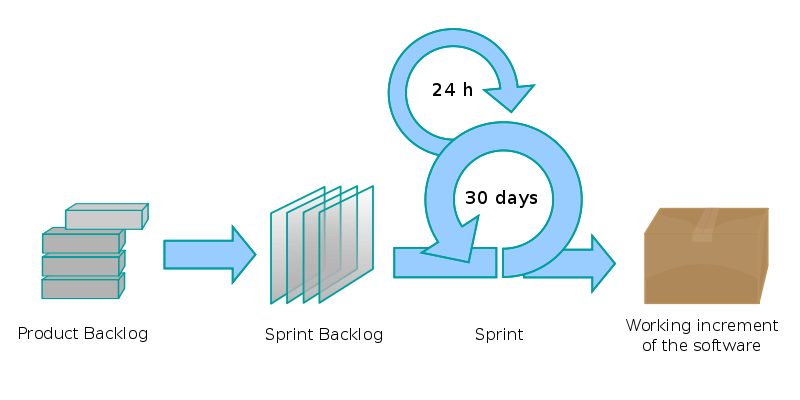
\includegraphics[scale=0.35]{immagini/scrum}
\caption{Diagramma del modello \emph{Scrum}. Immagine tratta da \href{https://it.wikipedia.org/wiki/Scrum_(informatica)}{Wikipedia}.}
\label{fig:scrum}
\end{figure}
\newpage
Questa metodologia consente e promuove un maggiore coinvolgimento del cliente rispetto a quelle tradizionali. Consente inoltre una maggiore flessibilità e reattività al cambio dei requisiti che possono avvenire in corso d'opera.
%***************************************************************************************




%***************************************************************************************
\section{Strumenti a supporto dei processi}
Questa sezione, illustra gli strumenti utilizzati a supporto dei processi e le tecnologie utilizzate per lo sviluppo.
\subsection{Gestione di progetto}
Per fornire assistenza ai clienti l'azienda utilizza Zendesk\footnote{\url{https://www.zendesk.it/}}, che è uno strumento che permette di centralizzare tutti i canali di comunicazione tra i quali \emph{social network}, \emph{email} e telefono. Inoltre fornisce una panoramica generale, della prestazione dell'assistenza e della soddisfazione del cliente.\\Per la gestione di progetto invece utilizza lo strumento Jira\footnote{\url{https://www.atlassian.com/software/jira}}, che fornisce degli strumenti per la gestione di sviluppo agile con il modello \emph{Scrum}, utilizzato nell'azienda. Nello specifico, Jira permette:
\begin{itemize}
\item Assegnazione dei \emph{ticket} tra i membri del \emph{team} di sviluppo;
\item Segnalazione di \emph{issue};
\item Integrazione con il sistema di \emph{repository};
\item Pianificazione dello \emph{sprint}.
\end{itemize}
\begin{figure}[h]
\centering
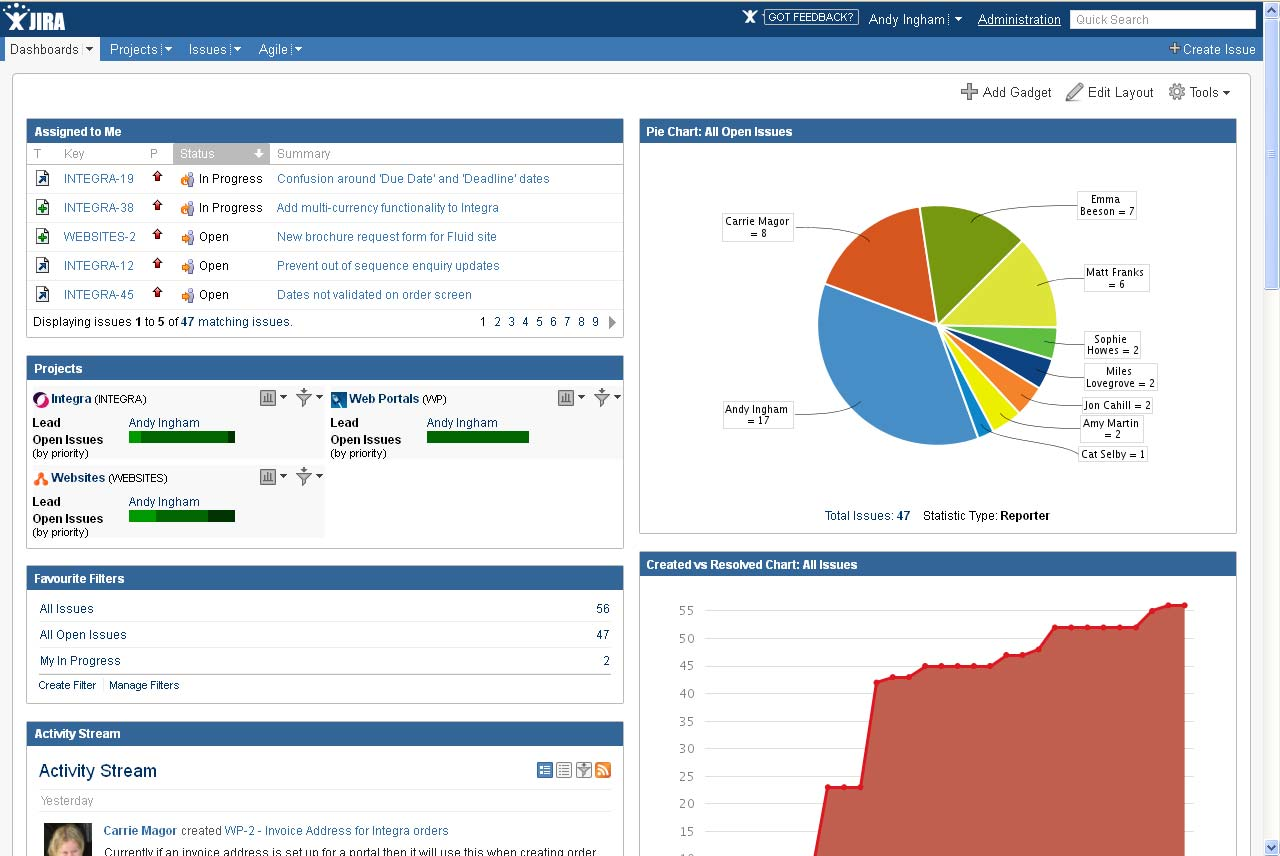
\includegraphics[scale=0.4]{immagini/jira}
\caption{Piattaforma di gestione di progetto Jira}
\label{fig:jira}
\end{figure}
Nextep non utilizza la \emph{Kanban Board} integrata in Jira, perché questo strumento di processo non è compatibile con la metodologia \emph{agile} in uso. Pertanto adopera una \emph{Scrum Board} fisica presente in ufficio.
\newpage
\subsection{Documentazione}
Nextep per la produzione documentale utilizza una serie di strumenti di Google Docs, per una serie di fattori tra i quali:
\begin{itemize}
\item Compatibilità con tutti i sistemi operativi utilizzati;
\item Permette di lavorare collaborativamente ai documenti;
\item Disponibilità;
\item Affidabilità.
\end{itemize}
\subsection{Sistema di versionamento}
Come sistema di versionamento, il \emph{team} utilizza lo strumento di Git\footnote{\url{https://git-scm.com/}}.\\I \emph{repository} sono gestiti in un \emph{server} locale, ed occasionalmente in server esterni.
\subsection{Ambiente di sviluppo}
A seconda del contesto, il \emph{team} utilizza l'ambiente di sviluppo che meglio si adatta alle tecnologie in uso nel progetto. In particolar modo adopera i seguenti \gls{ide}:
\begin{itemize}
\item Eclipse o IntelliJ: per lo sviluppo di applicazioni in Java e/o Scala;
\item Smultron/PhpStorm: per lo sviluppo di applicazioni in Php;
\item Sublime Text: per lo sviluppo in Html/Css, Javascript e Php.
\end{itemize}
\newpage
\subsection{Sistemi operativi}
L'azienda non impone nessun obbligo di utilizzo di un sistema operativo.\\I dipendenti utilizzano, a seconda delle preferenze, sistemi operativi quali Windows, Linux e MacOs. In particolar modo quest'ultimo, visto il recente investimento aziendale in nuovi terminali. Il fine è di incentivare i dipendenti, alla migrazione a questo sistema operativo.
\begin{figure}[h]
\centering
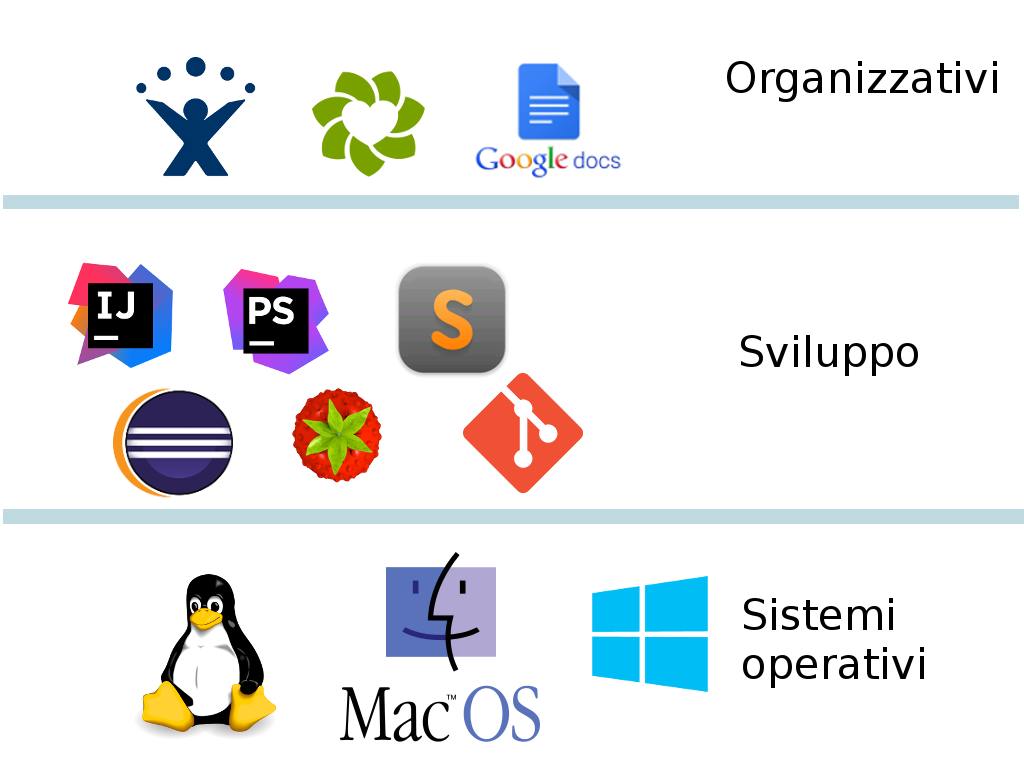
\includegraphics[scale=0.25]{immagini/strumenti}
\caption{Classificazione degli strumenti utilizzati}
\label{fig:strumenti}
\end{figure}
%********************************************************************************************




%********************************************************************************************
\section{Clientela tipo e propensione all’innovazione}
La tipologia di clientela per cui l'azienda lavora, copre una gamma che va dal singolo privato alle organizzazioni di grandi dimensioni.\\Essendo gli \emph{e-commerce} il \emph{core business} dell'azienda, Nextep lavora principalmente per aziende dell'ambito manifatturiero e rivendite.\\L'azienda lavora per clienti/aziende italiane e molto spesso per clienti della zona, visto il riconoscimento guadagnato nel padovano.\\Nextep riconosce questi valori guida da seguire:
\begin{itemize}
\item Attitudine all'innovazione per mantenere competitività;
\item Condivisione del \emph{know how} con le altre aziende in sede.
\end{itemize}
Questi principi rendono possibile un ambiente di \emph{co-working}, dove le 3 aziende della sede sperimentano e innovano, grazie alle conoscenze messe in condivisone. Per alimentare questa dinamica, l'azienda promuove periodicamente la formazione dei dipendenti, in modo che essi possano essere motivati e partecipi in questo ambiente. Visto l'importanza delle dinamiche personali, l'azienda organizza, al bisogno, degli incontri di \emph{team building} per avere sempre dei dipendenti in grado di lavorare in gruppo.  
%**************************************************************
             % L'azienda
% !TEX encoding = UTF-8
% !TEX TS-program = pdflatex
% !TEX root = ../tesi.tex
% !TEX spellcheck = it-IT

%**************************************************************
\chapter{Il progetto nella strategia aziendale}
\label{cap:il-progetto-nella-strategia-aziendale}
%**************************************************************
\intro{Questo capitolo fornisce una descrizione dettagliata del progetto di stage, e dei motivi che hanno spinto l'azienda a proporlo oltre che i benefici derivati da tale progetto. Vengono inoltre discussi i vincoli tecnologici e metodologici imposti.}\\




%**************************************************************************************************
\section{L'azienda e gli stage}
Questa sezione descrive il rapporto dell'azienda con gli stage e spiega quali sono i motivi che portano l'azienda a farli, in particolare per il progetto svolto.\\Data la forte evoluzione del settore \emph{web}, l'azienda persegue l'obiettivo di esplorare i nuovi segmenti del campo per mantenere un ruolo di rilievo nel mercato. Per questo motivo c'è l'esigenza di sperimentare continuamente nuove soluzioni, per valutare possibili impieghi e vantaggi. Si vengono quindi a creare le condizioni per un'opportunità di \emph{stage}, dove l'azienda richiede allo stagista una soluzione per le funzionalità richieste. Inoltre l'azienda sfrutta l'occasione degli \emph{stage} per valutare una possibile collaborazione e successivamente una assunzione in azienda nel caso che il soggetto sia valutato positivamente. Nel precedente \emph{stage}, visto l'interesse nel campo delle raccomandazioni, sono stati sviluppati dei prototipi che potessero soddisfare una raccomandazione utente in ambito \emph{e-commerce}. I sistemi di raccomandazione in ambito commerciale sono molto utili, perché permettono un guadagno dal punto di vista economico, e dal punto di vista della \emph{user experience} perché permettono di inserire pubblicità più pertinenti ai gusti dell'utente. In precedenza durante un recente \emph{stage}, l'azienda aveva sviluppato il modulo di raccomandazione denominato DRE, un sistema basato sul \emph{Collaborative filtering} che permette di fornire una raccomandazione in base alla somiglianza degli utenti.
\newpage
%**************************************************************************************************




%**************************************************************************************************
\section{Il progetto}
Questa sezione descrive il progetto di \emph{stage} e gli obiettivi che l'azienda ha fissato in relazione alle sue specifiche esigenze di mercato. 
\subsection{Il progetto}
Il progetto di stage consiste nella realizzazione di un sistema di raccomandazione basato sulla classificazione del comportamento degli utenti all'interno del sito. Il sistema deve poter permettere l'inserimento delle azioni dell'utente ogni volta che il suo comportamento ha prodotto un risultato. Una volta collezionata una considerevole mole di dati relativi ai comportamenti, il sistema deve poter fornire una raccomandazione all'utente sulla base del suo comportamento attuale. Il comportamento di un utente è descritto tramite una serie di iterazioni e il risultato raggiunto. A sua volta una iterazione è descritta tramite l'azione e l'oggetto su cui viene svolta. Questo comportamento viene poi elaborato dall'albero di decisione generato dai dati collezionati precedentemente. La generazione dell'albero si basa sull'algoritmo di classificazione ID3 (\emph{Iterative Dichotomiser 3}) che permette di selezionare l'attributo per discriminare il comportamento con il miglior guadagno informativo. Il sistema deve poter fornire una raccomandazione anche probabilistica nel caso di dati parziali sul suo comportamento.
\begin{figure}[ht]
\centering
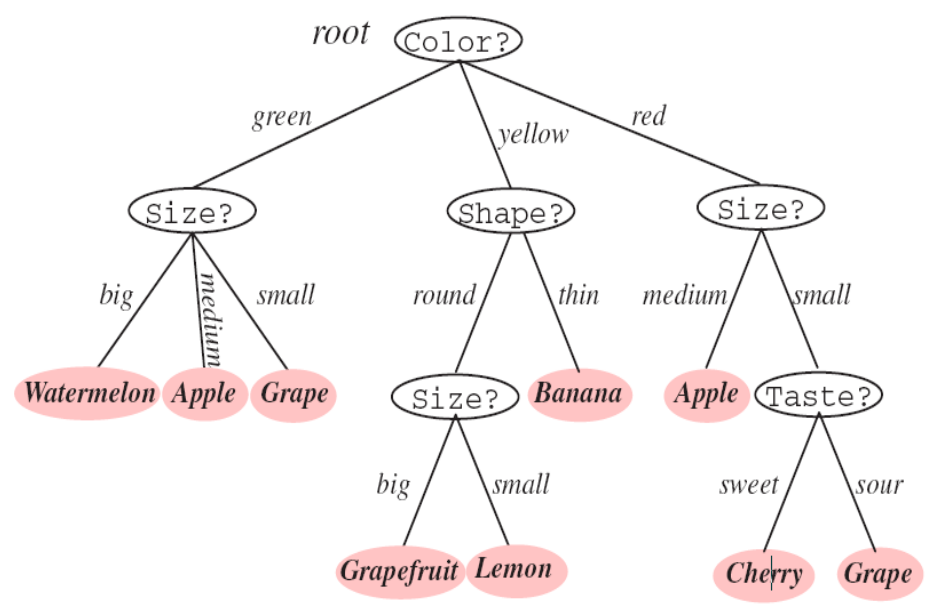
\includegraphics[scale=0.3,keepaspectratio]{tree}
\caption{Esempio di un albero decisionale}
\end{figure}
\subsection{Obiettivi}
Prima dell'inizio dello stage, Nextep ha redatto un \emph{Piano di Lavoro} contenente gli obiettivi da realizzare nelle settimane di \emph{stage}. Gli obiettivi erano suddivisi in minimi e massimi, successivamente in seguito ad una variazione delle priorità aziendali sono stati effettuati dei cambiamenti. Inizialmente, ho effettuato il \emph{porting} del modulo preesistente DRE, in modo che la persistenza fosse compatibile con OrientDb e che fosse compatibile con l'ultima versione di Play Framework. Visto il protrarsi delle attività di \emph{porting}, l'azienda ha deciso di sospendere il lavoro per poter lavorare sul nuovo modulo \emph{Tres}.
\newpage
Qui di seguito presento gli obiettivi dello stage:
\begin{itemize}
\item Obiettivi formativi
\begin{itemize}
\item Formazione sui sistemi di raccomandazione e degli algoritmi di apprendimento;
\item Studio delle tecnologie utilizzate, Scala e OrientDb;
\item Studio degli strumenti utilizzati, in particolar modo dei \emph{framework} e degli \emph{IDE}.
\end{itemize}
\item Obiettivi minimi
\begin{itemize}
\item Utilizzo del database OrientDb.
\end{itemize}
\item Obiettivi massimi
\begin{itemize}
\item Implementazione di nuovi modelli di algoritmi di apprendimento per migliorare l'individuazione dei gusti dell'utente;
\item Migliorare la fase di apprendimento del modello stesso;
\item Implementazioni di algoritmi di \emph{cluster} per il raggruppamento di elementi omogenei in un insieme di dati.
\end{itemize}
\end{itemize}
%**************************************************************************************************




%**************************************************************************************************
\section{Vincoli}
Questa sezione elenca i vincoli relativi al progetto di \emph{stage}.
\subsection{Vincoli temporali}
Per lo \emph{stage} i vincoli temporali sono imposti direttamente dall'università, essa stabilisce una durata minima di 300 ore e una durata massima di 320 ore. Per questo motivo ho modulato il \emph{Piano di Lavoro} in modo da distribuire le ore lavorative in 8 settimane. Con l'azienda ho concordato un impegno di 300 ore, divise in 37.5 ore settimanali. Le variazioni del piano sono state concordate con il \emph{tutor} aziendale in maniera da rispettare i vincoli temporali imposti in seguito a ritardi dovuti al \emph{porting} del modulo DRE.
\subsection{Vincoli metodologici}
Come strumento di versionamento ho scelto Git perché già utilizzato in precedenza e per il supporto che riceve da molti strumenti di sviluppo. Per la documentazione del codice ho scelto Scaladoc perchè viene fornito insieme al compilatore e similmente a Javadoc permette di documentare direttamente nel codice sorgente. Per il \emph{testing} nel progetto ho utilizzato TravisCI, esso fornisce un servizio di \emph{continuous integration} facilmente integrabile con i \emph{repository} di Github\footcite{https://github.com/}.
\begin{figure}[ht]
\centering
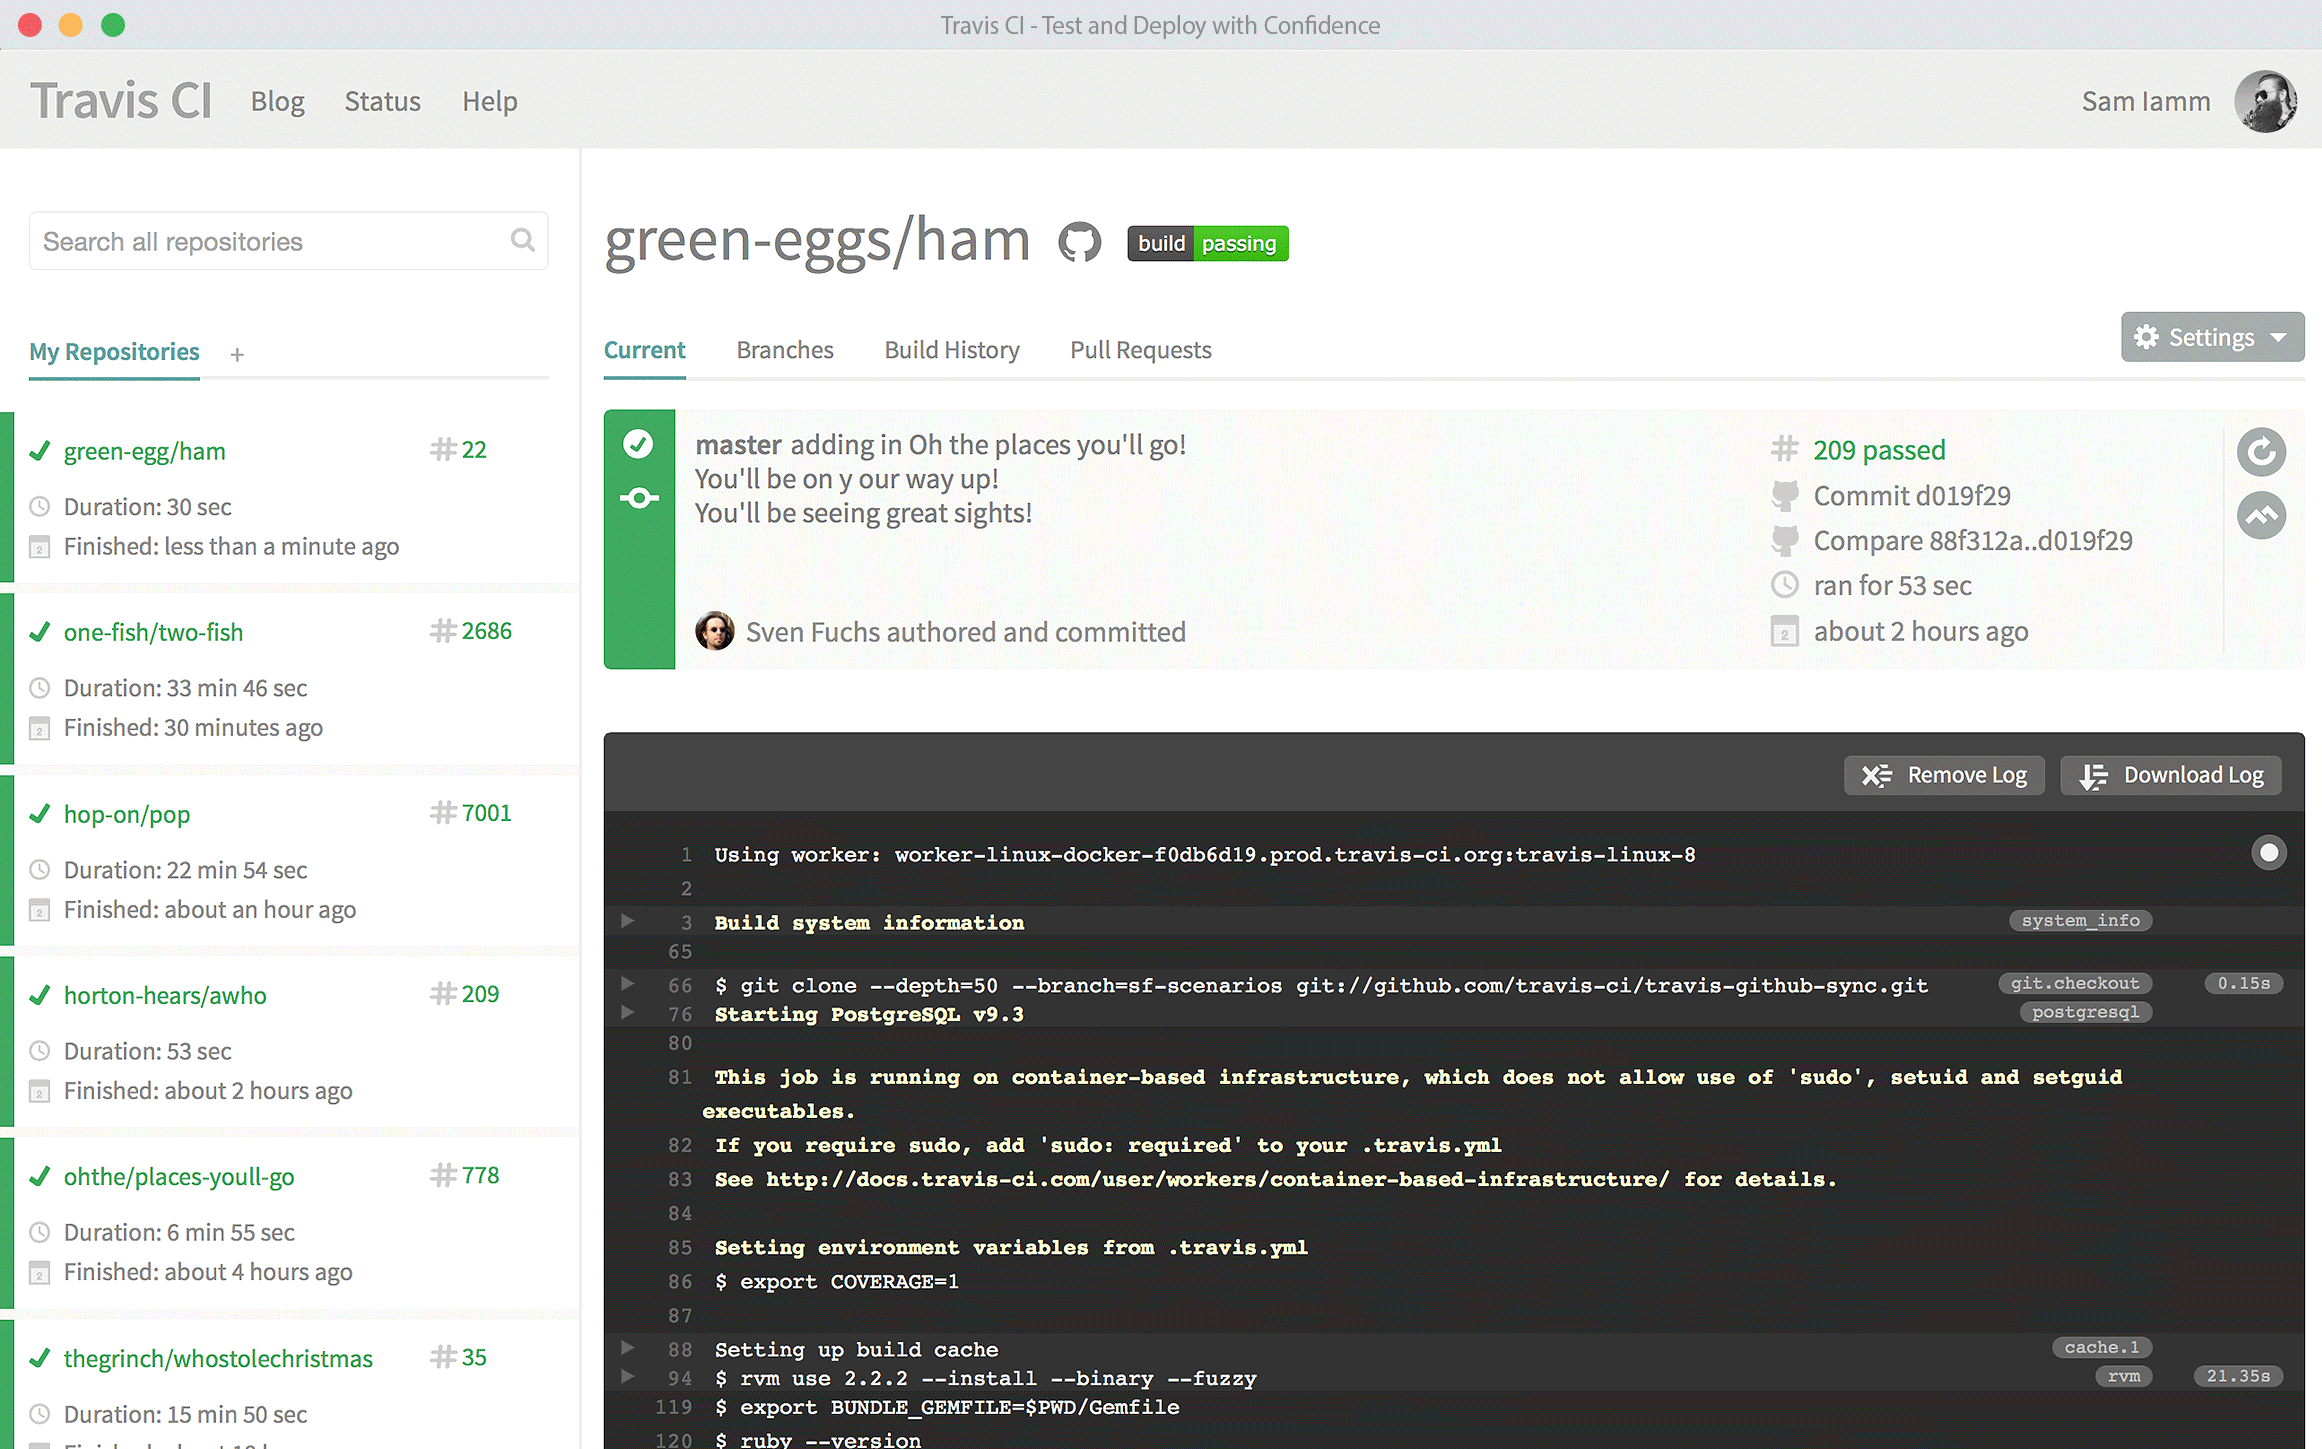
\includegraphics[scale=0.17,keepaspectratio]{travis}
\caption{Pannello di controllo travis}
\end{figure}
\newpage
Per lo sviluppo del codice ho scelto come \emph{IDE} IntelliJ in quanto:
\begin{itemize}
\item Già precedentemente utilizzato;
\item Ambiente di sviluppo compatibile con i maggiori linguaggi \emph{JVM-based};
\item Integrazione con Git;
\item Integrazione per lo sviluppo in Scala con Sbt.
\end{itemize}
Per la gestione progetti ho utilizzato il \emph{build tool} Sbt, perchè nell' ambiente di sviluppo di Scala è la scelta predominante ed è compatibile con il \emph{framework} utilizzato \emph{Play Framework}. Le caratteristiche distintive di questo \emph{framework} sono elencate di seguito:
\begin{itemize}
\item Definizione del file di configurazione in Scala;
\item Compatibilità con Scaladoc per documentazione;
\item Supporto per progetti misti Java/Scala;
\item Supporto per i maggiori \emph{tool} di \emph{testing};
\item Supporto per la gestione delle librerie.
\end{itemize}
Per la realizzazione dei diagrammi \emph{UML (Unified Modeling Language)} ho utilizzato Astah Professional\footcite{http://astah.net/}, uno strumento già utilizzato in precedenza e perché compatibile con gli ultimi standard \emph{UML 2.0}.
\subsection{Vincoli tecnologici}
\subsubsection{Scala}
Il principale linguaggio di programmazione adottato è Scala\footcite{http://www.scala-lang.org/} (acronimo di \emph{"Scalable Language"}). E' stato studiato per poter interoperare con \emph{Java Runtime Environment (JRE)}, quindi è possibile scrivere applicazioni sia in Java e Scala che eseguono nella stessa \emph{Java Virtual Machine (JVM)}. E' un linguaggio multi paradigma, che integra concetti provenienti dai linguaggi della programmazione ad oggetti e della programmazione funzionale. Scala è un linguaggio completamente \emph{object oriented}, infatti ogni elemento del linguaggio è un oggetto, compresi i tipi primitivi e le funzioni. Inoltre è un linguaggio funzionale, include funzioni di prima classe e una libreria con strutture dati immutabili efficienti.
\subsubsection{Play Framework}
Play è un \emph{framework} \emph{open source}, scritto in Java e Scala, che permette l'implementazione di \emph{web application} con il \emph{pattern model-view-controller}. Questo \emph{framework} trae ispirazione ed è simile a Ruby on Rails e Django.
\begin{figure}[ht]
\centering
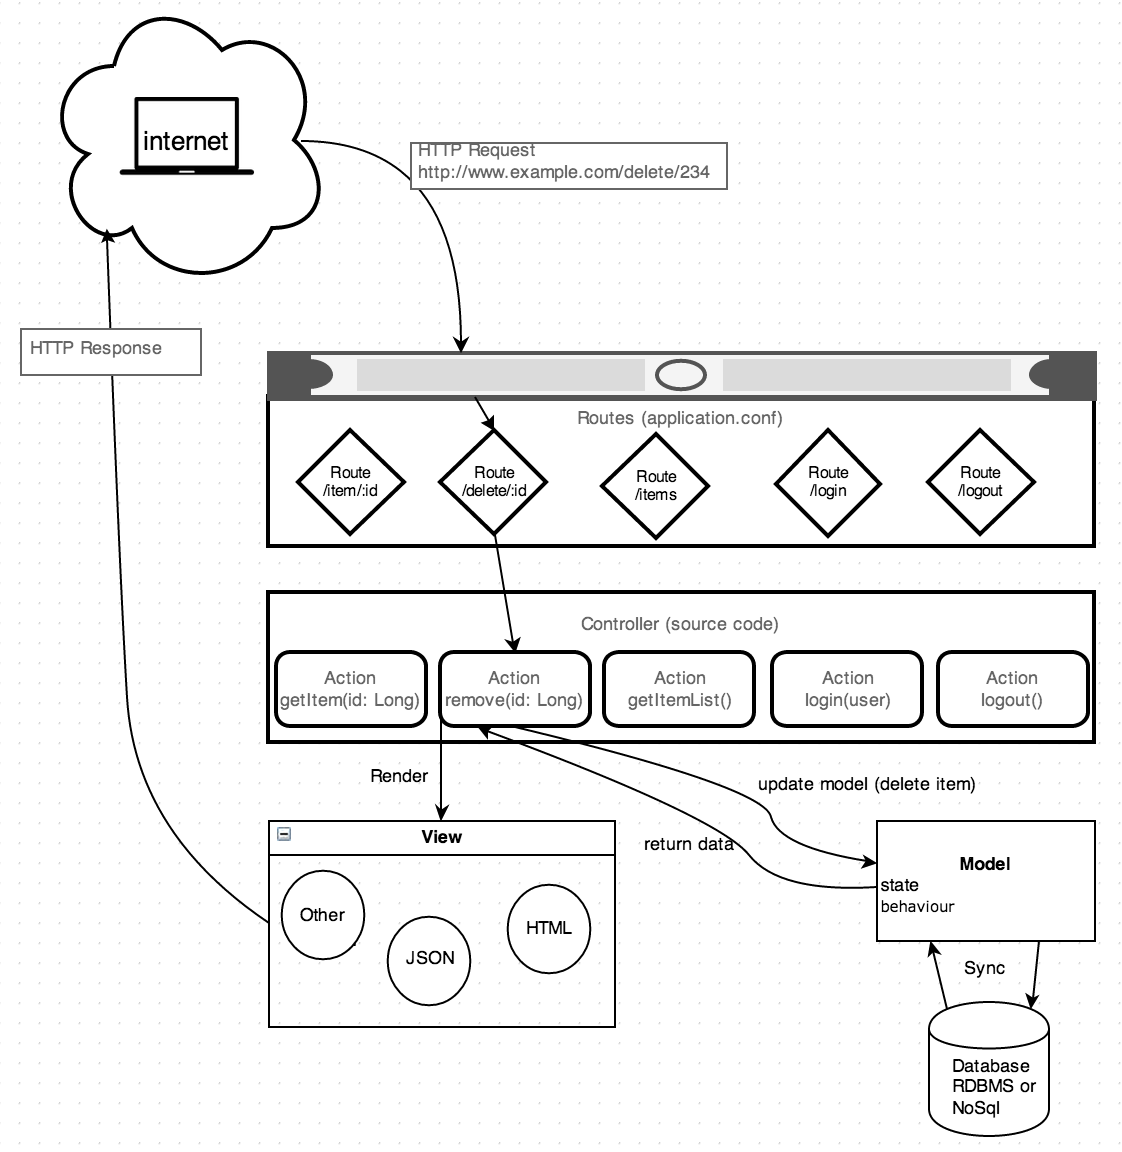
\includegraphics[scale=0.5]{immagini/play-arch}
\caption{Tipica architettura di un'applicazione che utilizza Play Framework. Immagine tratta da \href{https://110j.wordpress.com/2013/10/23/play-framework-2-1-architecture/}{Omer Haderi Blog}.}
\label{fig:play-app}
\end{figure}
\newpage
Le peculiarità che lo contraddistinguono dagli altri \emph{framework} sono le seguenti:
\begin{itemize}
\item Privo di stato: non viene mantenuta alcuna sessione sul server relativa ai dati dell'utente corrente;
\item Metodi statici: tutti i metodi dei \emph{controller} che vengono invocati dal \emph{framework} sono statici, o nel caso in cui si usi la versione Scala, sono funzioni di oggetti di Scala;
\item Gestione asincrona dell'\emph{input} e dell'\emph{output}: grazie all'uso di Netty Server, Play può gestire le richieste lunghe in modo asincrono;
\item Architettura modulare: come per Rails e Django, ci sono i moduli;
\item Supporto nativo per Scala: non solo Play è fatto internamente in Scala, ma espone anche delle interfacce Scala. Le interfacce Java sono state messe appositamente in \emph{package} diversi affinché possano seguire le convenzioni di Java.
\end{itemize}
Al suo interno permette una implementazione delle \emph{views}, specificando l'interfaccia con un linguaggio di \emph{markup} (e.g. Html, Xml, Json) in combinazione con del codice Scala. Vengono fornite molte classi di \emph{utility} come ad esempio Play Json Library che permette di operare con dei dati in formato Json, oppure un adattamento della libreria Specs2 che permette un supporto per il \emph{testing} di una applicazione in Play. Una tipica applicazione in Play funziona convogliando tutte le \emph{HTTP Request} nella componente \emph{Router} che invocherà a sua volta il \emph{Controller} pre-selezionato. Il \emph{Controller} interagisce con il \emph{Model} che a sua volta restituisce un risultato. In genere questo risultato verrà poi \emph{renderizzato} con la \emph{View} e fatto ritornare tramite un \emph{HTTP Response}.
\subsubsection{OrientDB}
Per la persistenza dei dati ho utilizzato OrientDb\footcite{http://orientdb.com/}, un \emph{Database Management System} (DBMS) multi-modello con una licenza \emph{open source}. Supporta i seguenti modelli di persistenza:
\begin{itemize}
\item \emph{Graph}: modello a grafo; 
\item \emph{Document}: modello a documenti come MongoDb;
\item \emph{Object}: modello ad oggetti che permette di memorizzare direttamente i \emph{POJO}.
\end{itemize}
Inoltre supporta modelli di definizione dello schema come \emph{schema-less}, \emph{schema-full} e \emph{schema-mixed}. Per motivi prestazionali non permette le \emph{join}, le relazioni sono gestite come in un database a grafo, ovvero delle connessioni dirette tra i \emph{record}. Questa caratteristica lo rende adatto nel contesto dei \emph{Big Data}, infatti la complessità computazionale per gestire una creazione di un \emph{link} è pari a O(1). Tra le caratteristiche più importanti di OrientDb:
\begin{itemize}
\item Scalabile: ovvero è possibile aggiungere al sistema un altro \emph{server} per aumentarne le prestazioni;
\item Transazionale: supporta transazioni completamente \emph{ACID} garantendo che tutte le transazioni  vengano processate in modo affidabile e nel caso di \emph{crash} viene ripristinato lo stato precedente(rollback);
\item Polyglot: supporta \emph{query} in un dialetto \emph{SQL-like}, oppure delle \emph{API REST} che forniscono l'accesso ai dati.
\end{itemize}
\begin{figure}[ht]
\centering
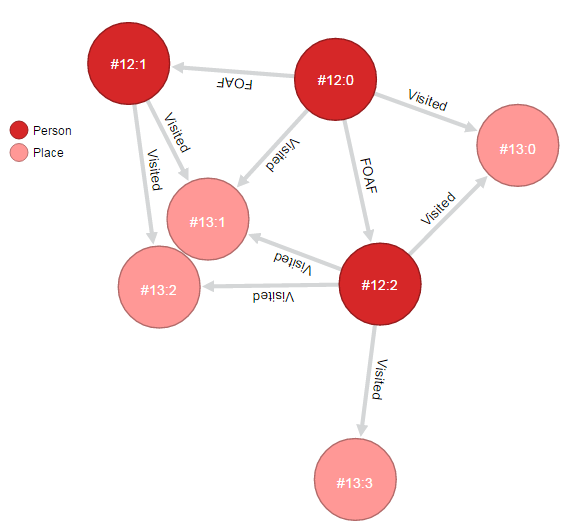
\includegraphics[scale=0.60]{immagini/graph_orientdb}
\caption{Esempio di modellazione in OrientDb. Immagine tratta da \href{http://blog.scalac.io/2015/11/26/orientdb-and-scala-part1.html}{Scalac Blog}}
\label{fig:orientdb-graph}
\end{figure}
%**************************************************************************************************




%**************************************************************************************************
\section{Obiettivi personali}
Questa sezione elenca gli obiettivi personali che hanno portato allo svolgimento dello \emph{stage}.\\Ho conosciuto l'azienda durante l'evento \emph{Stage-IT}. Questo evento mi ha dato la possibilità di approfondire molte proposte di \emph{stage}, da parte aziende provenienti da tutta la provincia di Padova e non. In seguito a tutte le proposte di \emph{stage} disponibili ho accettato la proposta di Nextep S.r.l. per i seguenti motivi:
\begin{itemize}
\item Il progetto permetteva di lavorare con tecnologie innovative che mi avrebbero fornito un valore professionale aggiunto;
\item Il progetto proposto era interessante perché toccava rami dell'intelligenza artificiale e dei sistemi di raccomandazione;
\item L'utilizzo di Scala, in modo da poter padroneggiare un linguaggio con un paradigma funzionale in forte ascesa di popolarità.
\end{itemize}
%**************************************************************************************************             % Il progetto nella strategia aziendale
% !TEX encoding = UTF-8
% !TEX TS-program = pdflatex
% !TEX root = ../tesi.tex
% !TEX spellcheck = it-IT

%**************************************************************
\chapter{Il progetto di stage}
\label{cap:il-progetto-di-stage}
%**************************************************************
\intro{Questo capitolo tratta dettagliatamente delle attività di pianificazione, studio, analisi, progettazione e sviluppo, svolte durante lo stage.}\\




%**************************************************************
\section{Organizzazione}
Per conseguire tutti gli obiettivi fissati, ho previsto un ammontare di 300 ore. Insieme al \emph{tutor} aziendale ho concordato la data di inizio stage il 5/10/2015 e la data di fine stage il 27/11/2015. Quindi un carico lavorativo di 37.5 ore settimanali, ovvero 7.5 ore giornaliere. 
\begin{figure}[h]
\centering
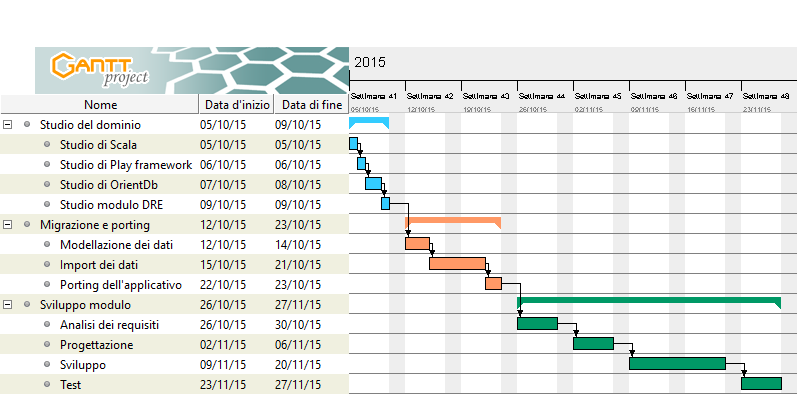
\includegraphics[scale=0.52]{immagini/gantt}
\caption{Suddivisione delle attività}
\label{fig:gantt}
\end{figure}
\newpage
\subsection{Pianificazione}
In sede di pianificazione, prima dell'inizio dello \emph{stage}, ho programmato 3 macro attività sequenzialmente. Ho assegnato, nel primo periodo, una settimana per l'attività di studio del dominio, in quanto questa attività è propedeutica alle successive attività. Nel periodo successivo di 2 settimane, ho pianificato l'attività di \emph{porting} dell'applicativo DRE, su richiesta del \emph{tutor} per motivi di strategia aziendale. Nell'ultimo periodo, ho programmato l'attività di sviluppo del modulo denominato Tres. Ho privilegiato quest'ultima attività, assegnando un totale di 5 settimane lavorative. Qui di seguito illustro le sotto-attività programmate per ogni settimana. 
\begin{itemize}
\item \textbf{Prima settimana:}
\begin{itemize}
\item Studio del \emph{database} OrientDB;
\item Studio del linguaggio di programmazione Scala;
\item Studio del \emph{framework} Play;
\item Studio del progetto preesistente;
\end{itemize}
\item \textbf{Seconda e terza settimana:} migrazione dalla tecnologia MongoDB a OrientDB e \emph{porting} all’ultima versione di Play;
\item \textbf{Quarta settimana:} Analisi dei requisiti del nuovo modulo;
\item \textbf{Quinta settimana:} progettazione architetturale;
\item \textbf{Sesta e settima settimana:} implementazione modulo;
\item \textbf{Ottava settimana:} test.
\end{itemize}
La figura \hyperref[fig:gantt]{3.1} presenta il diagramma di \emph{gantt} utilizzato per la pianificazione.
%**************************************************************




%**************************************************************
\section{Analisi dei requisiti} 
\subsection{Requisiti}
Per l'attività di analisi dei requisiti, ho svolto molteplici incontri insieme al \emph{tutor} aziendale, per delineare quali funzionalità dovesse offrire il sistema. Il \emph{tutor} mi ha fornito molti esempi ed illustrazioni, per capire al meglio quali requisiti il sistema dovesse soddisfare. Tuttavia questa attività è stata molto ostica, perché sia il \emph{tutor} e sia il \emph{CEO} esprimevano richieste diverse e spesso molto discordanti. Visto che il proponente non aveva una visione chiara sul sistema da implementare, ho cercato di assumere un atteggiamento più propositivo, per aiutarlo a comprendere i suoi bisogni e portare a termine l'analisi dei requisiti nei tempi prefissati. Una volta definito le funzionalità, ho trascritto i requisiti in un file testuale, in un formato organizzato tabellare. Visto le dimensioni ridotte del progetto ho prediletto il tracciamento dei requisiti con un file di testo anziché utilizzare un sistema automatizzato. Il file è stato poi sottoposto a versionamento all'interno del \emph{repository}, per permettere operazioni di consultazione e modifica all'evolversi dei requisiti. La notazione scelta per suddividere i requisiti è la seguente: 
\begin{center}
R[Importanza][Tipologia][Codice]
\end{center}
\newpage
\begin{itemize}
\item Importanza può assumere i seguenti valori:
\begin{itemize}
\item \textbf{OBB:} requisito obbligatorio. Il soddisfacimento è necessario per il raggiungimento degli obiettivi dello \emph{stage};
\item \textbf{DES:} requisito desiderabile. L'implementazione non è fondamentale, ma dà valore aggiunto al prodotto.
\end{itemize}
\item Tipologia può assumere i seguenti valori:
\begin{itemize}
\item \textbf{F:} requisiti funzionali. Specifica una funzionalità che il \emph{software} deve avere;
\item \textbf{V:} requisiti di vincolo. Specifica il vincolo che il \emph{software} deve avere;
\item \textbf{P:} requisiti di prestazione. Specifica un vincolo di \emph{performance} che il \emph{software} deve fornire.
\end{itemize}
\item Codice è un \emph{id} numerico univoco.
\end{itemize}
\begin{figure}[h]
\centering
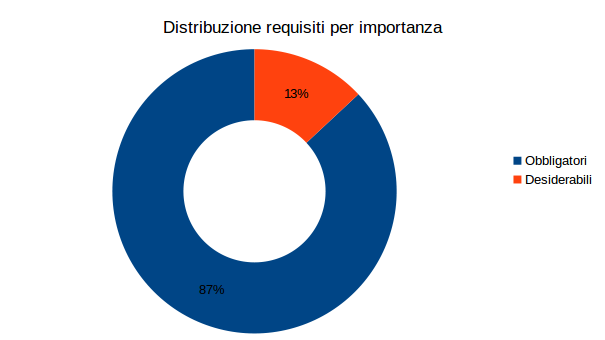
\includegraphics[scale=0.72]{immagini/distribuzionereqi}
\caption{Distribuzione requisiti in percentuale per tipologia}
\label{fig:distr-req-tip}
\end{figure}
Durante l'analisi dei requisiti, prima di trasporre i requisiti secondo la notazione precedentemente menzionata, ho rielaborato i requisiti. In modo che essi non contenessero ambiguità verbali, se presenti ho corredato al documento di analisi un glossario, dove specificare i termini ed evitare così interpretazioni errate del requisito. Inoltre ho suddiviso ogni requisito in più requisiti, fino a che ogni singolo requisito risultasse indivisibile. Invece i requisiti che risultavano ridondanti tra loro, li ho uniti affinché ogni requisito risultasse indipendente. Ho verificato che ogni requisito fosse verificabile secondo una metrica in modo da certificarne il soddisfacimento. Al termine dell'analisi, i requisiti individuati ammontano a 23. Come raffigurato nell'immagine \ref{fig:distr-req-tip}, i requisiti sono 15 di natura funzionale, 1 prestazionale e i restanti 7 requisiti di vincolo. I requisiti sono stati classificati per priorità, determinando così 20 requisiti obbligatori e 3 desiderabili. I requisiti desiderabili riguardano nella maggior parte gli obiettivi di massima fissati dal piano di lavoro. %I requisiti obbligatori sono stati ordinati secondo i criteri di stabilità (ovvero il numero di modifiche attese) e il grado di necessità (essenziale, condizionale, opzionale) 
\begin{figure}[h]
\centering
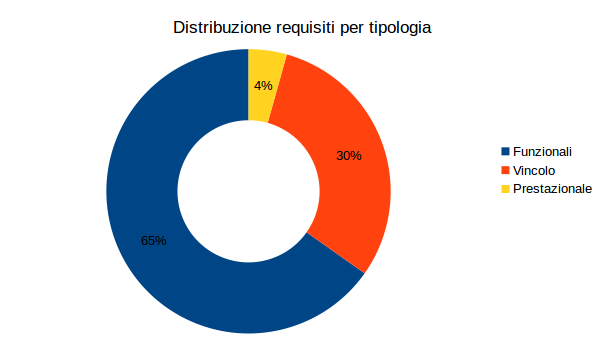
\includegraphics[scale=0.72]{immagini/distribuzionereqt}
\caption{Distribuzione requisiti in percentuale per importanza}
\label{fig:distr-req-imp}
\end{figure}

%Tabella requisiti:
%\def\arraystretch{1.8}
%\begin{longtable}{|l|p{7cm}|}
%\hline
%\textbf{Codice} &	\textbf{Descrizione}	\\\hline
%ROBBF1	&	Il sistema deve permettere l'inserimento di un nuovo comportamento	\\\hline
%ROBBF2	&	Il sistema deve restituire un messaggio di segnalazione in caso di errore durante il salvataggio \\\hline
%ROBBF3	&	I dati ricevuti devono essere in formato Json \\\hline
%ROBBF4	&	I dati inviati devono essere in formato Json \\\hline
%ROBBF5	&	Il sistema deve restituire un messaggio di errore in caso di Json non valido \\\hline
%ROBBF6	&	Devono essere inseriti almeno 100 comportamenti per produrre la raccomandazione \\\hline
%ROBBF7	&	Il sistema deve restituire un messaggio di conferma quando l'algoritmo è pronto a produrre una raccomandazione	\\\hline
%ROBBF8	&	Il sistema deve permettere il calcolo dell'entropia del \emph{dataset} \\\hline
%ROBBF9	&	Il sistema deve permettere il calcolo del guadagno di informazione del \emph{dataset}	\\\hline
%ROBBV10	&	Il sistema deve permettere la costruzione ricorsivamente dell'albero di decisione	\\\hline
%ROBBV11	&	Il sistema deve permettere la creazione di tanti nodi quanti sono i possibili valori dell'attributo scelto \\\hline
%ROBBV12	&	L'algoritmo di costruzione dell'albero deve fermarsi quando tutte le istanze di un nodo appartengono alla stessa classe \\\hline
%ROBBF13	&	Il sistema deve permettere di ricevere una richiesta per classificare un comportamento vuoto \\\hline
%ROBBF14	&	Il sistema, per la richiesta con un comportamento vuoto, deve restituire tutte le raccomandazioni con le percentuale calcolate in base al \emph{dataset} \\\hline
%ROBBF15	&	Il sistema deve permettere di classificare un comportamento dell'utente \\\hline
%ROBBF16	&	Il sistema deve fornire una raccomandazione o più in base alla classificazione del comportamento \\\hline
%ROBBF17	&	Il sistema deve fornire insieme alla raccomandazione la percentuale di adeguatezza	\\\hline
%ROBBV18	&	Il sistema deve permettere la modifica dell'albero di decisione ogni 24 ore	\\\hline
%ROBBV19	&	Devono essere rispettate le metriche sulla stesura del codice riportate nella sezione 3.5 \\\hline
%RDESF20	&	Devono essere implementati nuovi algoritmi basati sulla teoria de giochi	\\\hline
%RDESV21	&	Devono essere implementati nuovi algoritmi di \emph{clustering}	\\\hline
%RDESV22	&	Deve essere sviluppato il pannello di amministrazione	\\\hline
%ROBBP23	&	Il \emph{database} deve essere in grado di memorizzare almeno 100.000 record al secondo	\\\hline
%\caption{Tabella dei requisiti}
%\end{longtable}
\newpage
\subsection{Casi d'uso}
Durante l'analisi dei requisiti ho realizzato dei diagrammi \gls{uml}, utilizzando il \emph{software} Astah. Tres è concepito per operare con Bdrim, una piattaforma di raccolta dati sviluppato in collaborazione con Allos. Quindi l'unico attore coinvolto nell'utilizzo di Tres è Bdrim, che espone un caso d'uso principale. In questa sezione riporto i casi d'uso principali, che descrivono maggiormente il sistema nel suo complesso. Per ogni caso d'uso ho specificato: 
\begin{itemize}
\item Gli attori coinvolti;
\item Pre e post condizione;
\item Scopo e descrizione;
\item Flusso principale degli eventi.
\end{itemize}
Inoltre, se previsto, ho specificato estensione e lo scenario alternativo.
\newpage
\subsubsection{UC0}
\begin{figure}[h]
\centering
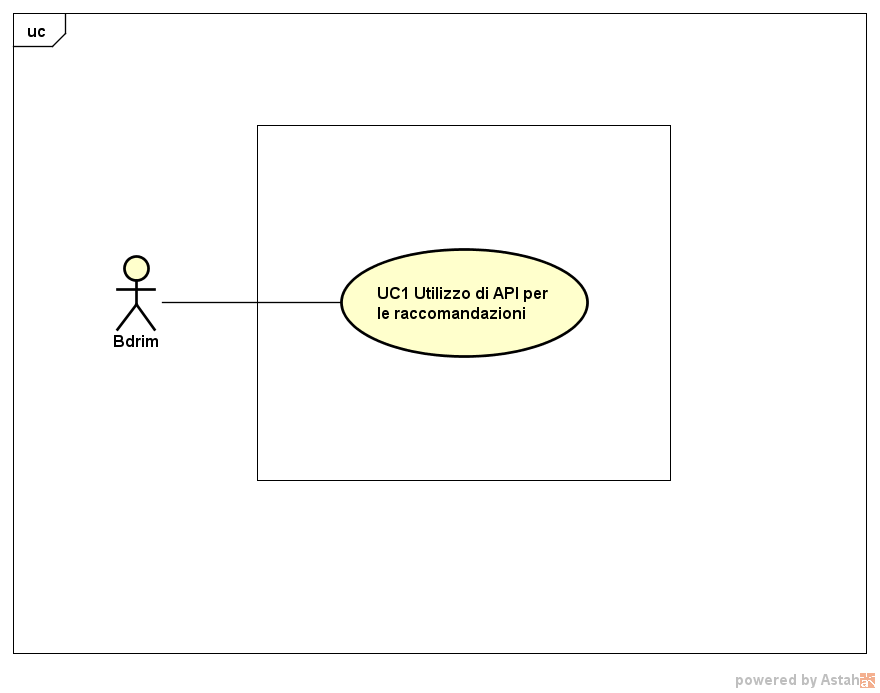
\includegraphics[scale=0.42]{immagini/UC0a}
\caption{UC0: Tres}
\label{fig:UC0}
\end{figure}
\begin{itemize}
\item \textbf{Attori:} Bdrim
\item \textbf{Scopo e descrizione:} Questo caso d'uso descrive le funzionalità messe a disposizione dal sistema. Principalmente Bdrim può usufruire delle \gls{api} per le raccomandazioni fornite da Tres.
\item \textbf{Pre-condizione:} Il \emph{server} è stato avviato.
\item \textbf{Flusso principale degli eventi:} Bdrim utilizza le \gls{api} per ottenere una raccomandazione.
\item \textbf{Post-condizione:} Il sistema risponde alle richieste HTTP effettuate da Bdrim.
\end{itemize}
\newpage
\subsubsection{UC1}
\begin{figure}[h]
\centering
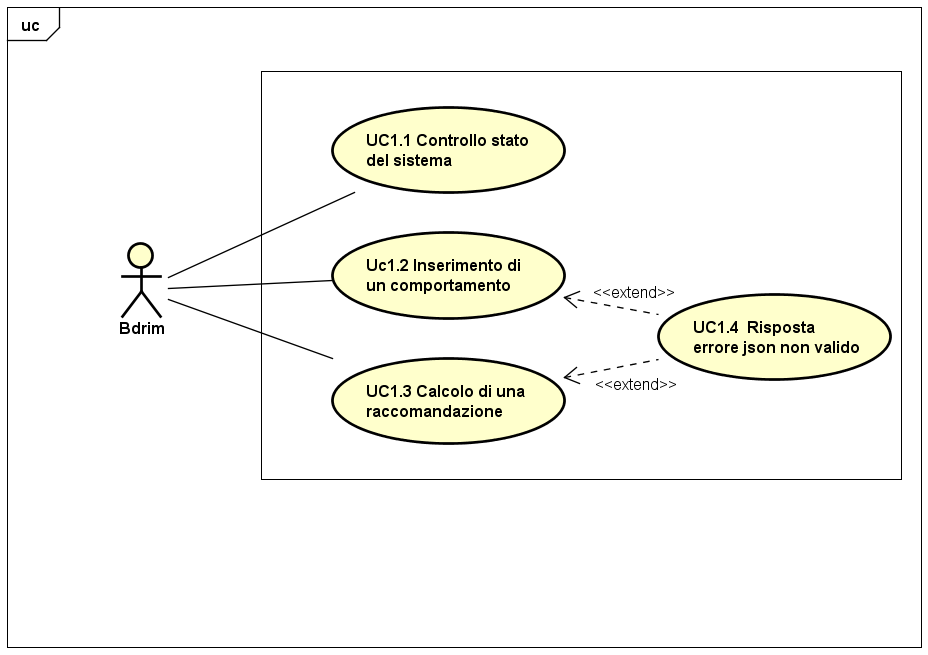
\includegraphics[scale=0.42]{immagini/UC1a}
\caption{UC1: Tres}
\label{fig:UC1}
\end{figure}
\begin{itemize}
\item \textbf{Attori:} Bdrim
\item \textbf{Scopo e descrizione:} Questo caso d'uso illustra le funzionalità offerte dal sistema a Bdrim. Bdrim ha la possibilità di effettuare delle richieste \gls{rest} al sistema;
\item \textbf{Pre-condizione:} Il \emph{server} è stato avviato e Tres è stato attivato.
\item \textbf{Flusso principale degli eventi:}
\begin{itemize}
\item[1] Bdrim richiede lo stato del sistema [UC1.1];
\item[2] Nel caso il sistema sia pronto Bdrim richiede la raccomandazione[UC1.3];
\item[3] Bdrim può inserire un comportamento[UC1.2].
\end{itemize}
\item \textbf{Scenario alternativo:} Bdrim effettua delle richieste \emph{HTTP}, inviando un oggetto \gls{json} malformato, oppure invalido. Il sistema ritorna una risposta \emph{HTTP} che segnala l'errore in formato \gls{json}. 
\item \textbf{Estensione:} Bdrim riceve una risposta \emph{HTTP} contenente un \gls{json}, che segnala l'errore di dati non validi [UC1.4];
\item \textbf{Post-condizione:} Il sistema risponde alle richieste \emph{HTTP}, ritornando una risposta \emph{HTTP}. I dati ritornando in formato \gls{json}.
\end{itemize}
%**************************************************************




%**************************************************************
\newpage
\section{Progettazione architetturale}
Questa sezione descrive l'attività di progettazione. Illustra l'architettura generale del sistema, le relazioni interne, la struttura del \emph{database} e infine i \emph{design pattern} utilizzati.
\subsection{Visione ad alto livello}
Il contesto di utilizzo dell'applicativo è la piattaforma di Bdrim. Questa piattaforma permette di gestire nuovi moduli, per introdurre nuove funzionalità. Ogni modulo deve essere assolutamente isolato, per poter essere facilmente modificabile e interscambiabile con altri moduli, che migliorino le sue funzionalità. Quindi la visione generale del sistema, si riconduce ad un modello \emph{client-server} dove i ruoli sono:
\begin{itemize}
\item \textbf{Server:} rappresentato da Tres, elabora le richieste \emph{HTTP} ricevute da Bdrim.
\item \textbf{Client:} rappresentato unicamente da Bdrim.
\end{itemize}
%\begin{figure}[h]
%\centering
%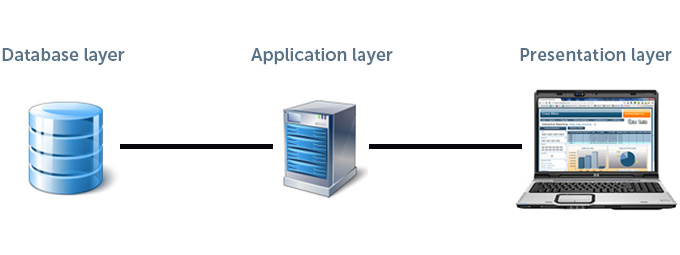
\includegraphics[scale=0.42]{immagini/client-server}
%\caption{Visione generale architettura \emph{client-server}. Immagine tratta da \href{http://%contentdeliverance.com/2011/client-server-architecture/}{Content Deliverance}}
%\label{fig:client-server}
%\end{figure}
\begin{figure}[h]
\centering
\includegraphics[scale=0.50]{immagini/architetturagenerale}
\caption{Visione generale dell'architettura}
\label{fig:arch-gen}
\end{figure}
Le due componenti sono indipendenti tra loro e comunicano utilizzando una architettura \gls{rest}.
\newpage
\subsection{Architettura}
Per la realizzazione di Tres, ho seguito un \emph{design} architetturale \gls{mvc}. Quindi i \emph{package} principali sono: \emph{model}, \emph{view} e \emph{controller}. Attualmente il \emph{package} \emph{views} non viene utilizzato. Esso tornerà utile in eventuali sviluppi successivi, per la creazione di una interfaccia di amministrazione per Bdrim o altre eventuali funzionalità. Qui di seguito illustro la visione generale e successivamente le componenti del sistema.  
\begin{figure}[h]
\centering
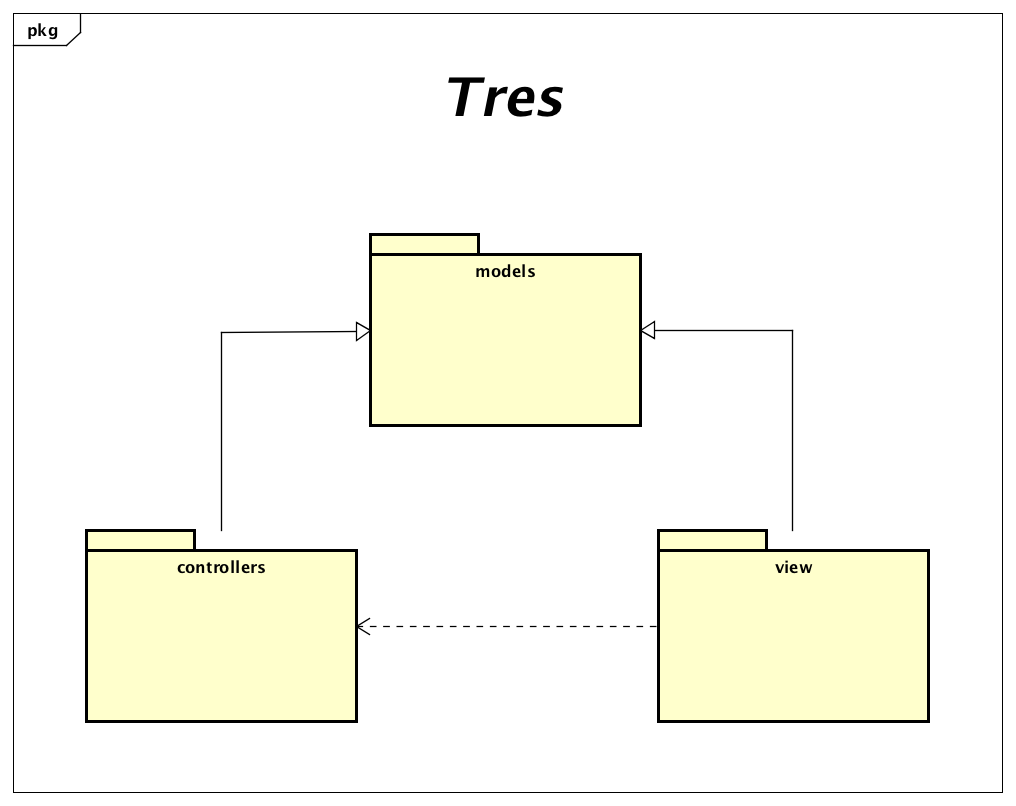
\includegraphics[scale=0.35]{immagini/architetturamvc}
\caption{Diagramma del \emph{package} \emph{tres}}
\label{fig:pack-tres}
\end{figure}
\newpage
\subsubsection{controllers}
Il \emph{package} \emph{controllers}, contiene le componenti responsabili della logica di controllo e nello specifico contiene due classi. \emph{BridgeController} è la componente che gestisce le richieste \emph{HTTP}, instradate dalla componente \emph{router} di Play. Il \emph{package} interagisce con \emph{models}, utilizzando i servizi messi a disposizione e le rappresentazioni dei dati.
\begin{figure}[h]
\centering
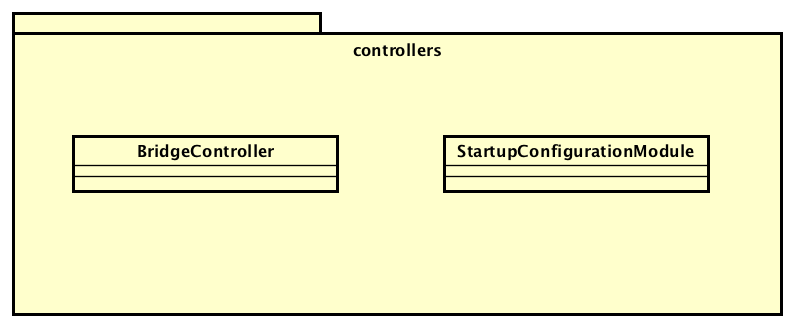
\includegraphics[scale=0.35]{immagini/controllers}
\caption{Diagramma del \emph{package} \emph{controllers}}
\label{fig:pack-controller}
\end{figure}
\subsubsection{models}
Il \emph{package} \emph{models}, contiene tutta la logica di \emph{business} del sistema e di accesso ai dati. E' responsabile di fornire una separazione, dalla rappresentazione interna dei dati del database. Fornisce tutte le interfacce necessarie al \emph{controller} per fornire i servizi.
\begin{figure}[h]
\centering
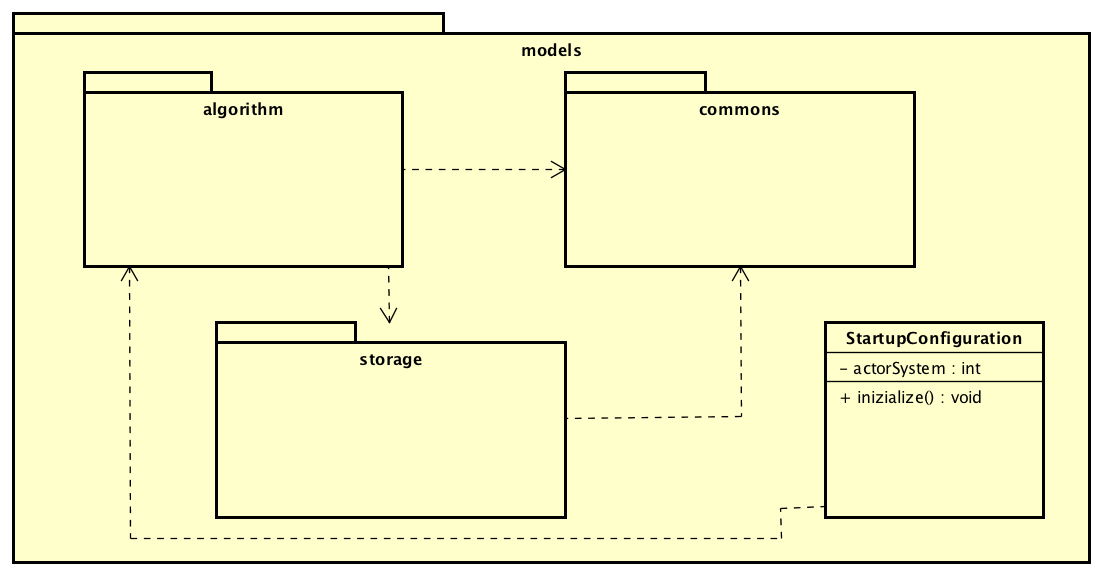
\includegraphics[scale=0.30]{immagini/models}
\caption{Diagramma del \emph{package} \emph{models}}
\label{fig:pack-models}
\end{figure}
\paragraph{Classi contenute}
\begin{itemize}
\item \textbf{StartupConfiguration:} Questa classe è responsabile di schedulare la generazione dell'albero, per le raccomandazioni. La generazione dell'albero avviene ogni 24 ore, solamente se sono disponibili almeno 100 comportamenti memorizzati.
\end{itemize}
\paragraph{Package contenuti}
\paragraph*{commons}
Il \emph{package} \emph{commons} contiene le componenti per la rappresentazione interna dei dati. All'interno sono presenti dei convertitori impliciti, che permettono la validazione e la conversione in formato \gls{json}. Funzionalità utili per le componenti nel \emph{controllers}. 
\begin{figure}[h]
\centering
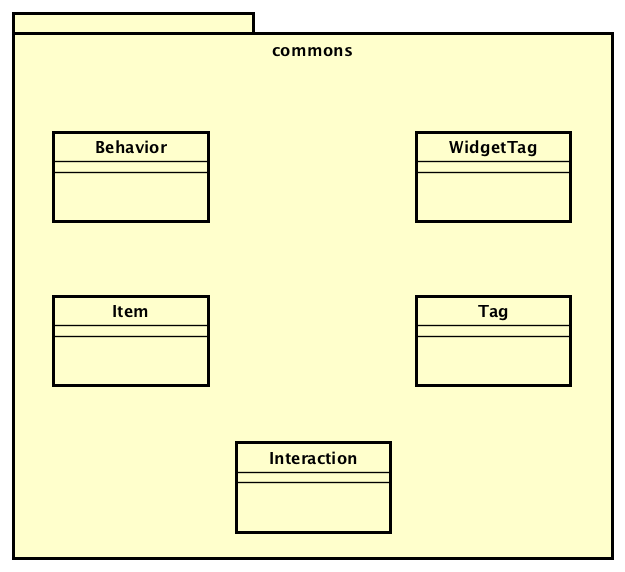
\includegraphics[scale=0.28]{immagini/commons}
\caption{Diagramma del \emph{package} \emph{commons}}
\label{fig:pack-commons}
\end{figure}
\paragraph*{storage}
Il \emph{package} \emph{storage} è responsabile dell'accesso ai dati. Fornisce una interfaccia per le funzionalità \emph{CRUD}. Il \emph{package} dipende dalle componenti in \emph{commons}, e per ognuna implementa l'interfaccia per l'interazione con OrientDb. Le componenti che gestiscono la persistenza in OrientDb utilizzano le \gls{api} Blueprints\footcite{https://github.com/tinkerpop/blueprints}, perchè OrientDb aderisce a questo standard di default. TinkerPop Blueprints fornisce delle \gls{api} per manipolare \emph{database} a grafo ed è incluso nello \emph{stack} dei progetti di TinkerPop\footcite{http://tinkerpop.incubator.apache.org/}
\begin{figure}[h]
\centering
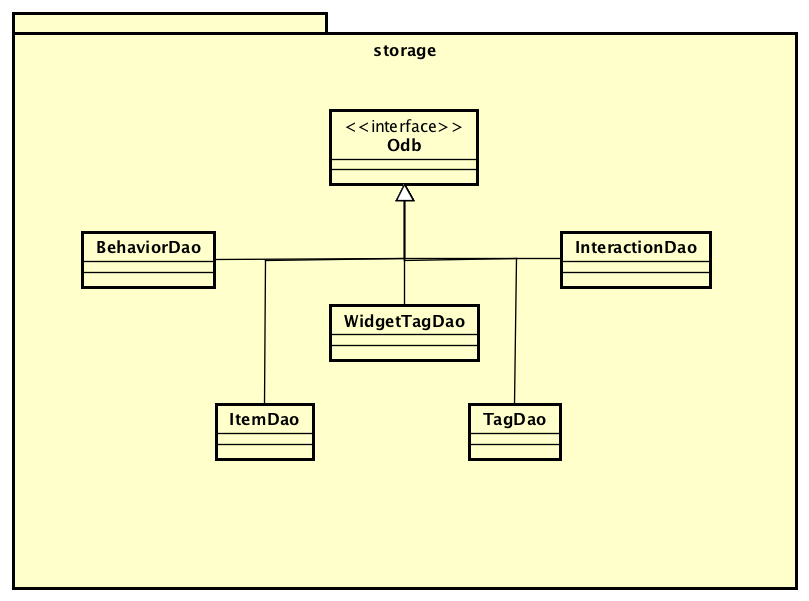
\includegraphics[scale=0.28]{immagini/storage}
\caption{Diagramma del \emph{package} \emph{storage}}
\label{fig:pack-storage}
\end{figure}
\newpage
\paragraph*{algorithm}
Il \emph{package} \emph{algorithm}, contiene le componenti \emph{software} che realizzano l'algoritmica, basata essenzialmente su \emph{ID3} ed è fortemente dipendente dalle componenti presenti in \emph{commons}. Fornisce la funzionalità per la costruzione dell'albero decisionale, sulla base dei \emph{behavior} in \emph{input}. Offre la funzionalità per ricevere in \emph{output} la raccomandazione, sulla base di un \emph{behavior} in \emph{input}.
\begin{figure}[h]
\centering
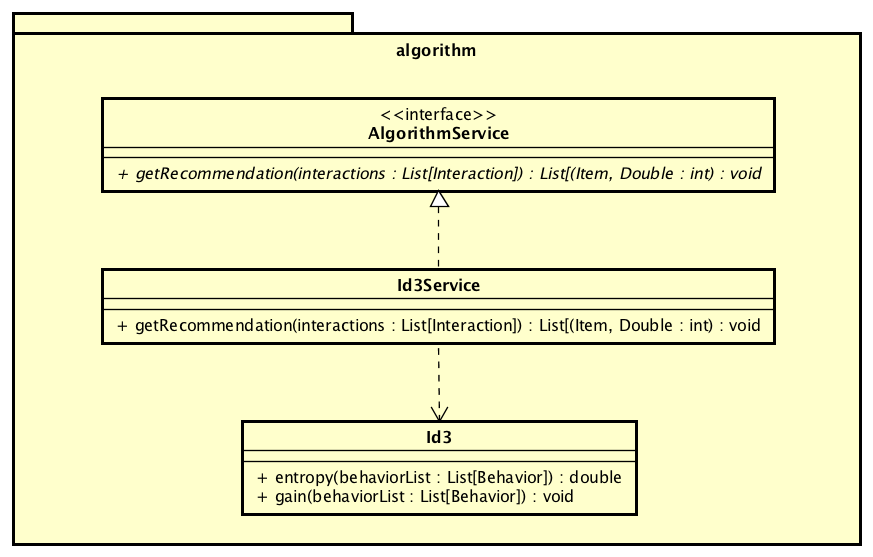
\includegraphics[scale=0.30]{immagini/algorithm}
\caption{Diagramma del \emph{package} \emph{algorithm}}
\label{fig:pack-algorithm}
\end{figure}
\subsection{Database}
Rispetto alle esperienze precedenti, come nel mio corso di laurea dove ho utilizzato tecnologie più tradizionali come i \emph{database} relazionali. Questa occasione mi ha permesso di utilizzare un database \emph{NoSQL}, come OrientDb. Questo \emph{database} supporta diversi modelli di persistenza. Per questo progetto ho utilizzato il modello a grafo, che fa riferimento direttamente alla \emph{teoria dei grafi}. In particolare la variante di grafo che OrientDb utilizza è \emph{property graph}. Per la modellazione ho tenuto presente i seguenti concetti:
\begin{itemize}
\item I vertici sono delle entità, mentre gli spigoli rappresentano le relazioni;
\item Una entità contiene un chiave identificativa e delle proprietà; 
\item Una relazione può contenere delle proprietà, è espressa tramite una \emph{label} e collega due entità. La direzione della relazione è importante per la semantica della relazione.
\end{itemize}
In OrientDb è possibile aggiungere attributi agli spigoli, ma è fortemente sconsigliato per motivi prestazionali\footnote{http://orientdb.com/docs/last/Performance-Tuning-Graph.html}. Per la persistenza dei dati ho scelto una definizione dei dati di tipo \emph{schema-full}, per evitare un controllo dei dati a \emph{run-time} nelle componenti del \emph{package} \emph{storage}.
\newpage
\begin{figure}[h]
\centering
\includegraphics[scale=0.50]{immagini/databaseschema}
\caption{Modello a grafo del database}
\label{fig:database-schema}
\end{figure}
La fase di modellazione a grafo è simile alla tecnica di modellazione relazionale. All'inizio ho individuato le entità del dominio e le modalità con cui si relazionano. Successivamente, invece di trasformare la rappresentazione in tabelle, ho arricchito lo schema andando ad individuare gli attributi interni delle entità e delle relazioni. Le entità principali che ho individuato sono:
\begin{itemize}
\item \textbf{Behavior:} questa entità rappresenta il comportamento di un utente all'interno di un sito web.
\item \textbf{Item:} questa entità rappresenta in genere un oggetto in vendita nel sito web.
\item \textbf{WidgetTag:} questa entità rappresenta un elemento generico all'interno di un sito web. Serve per individuare l'oggetto su cui l'utente svolge una azione.
\item \textbf{Tag:} questa entità è una etichetta generica, che serve a descrivere un \emph{Item}.
\end{itemize}
Le relazioni individuate sono:
\begin{itemize}
\item \textbf{Interaction:} Questa relazione parte dalla entità \emph{Behavior} e arriva a \emph{WidgetTag}. Esprime principalmente che un \emph{Behavior} ha interagito sul \emph{WidgetTag} collegato, con una azione specifica;
\item \textbf{Result:} Questa relazione parte da entità \emph{Behavior} e arriva a \emph{Item}. Esprime il risultato di un \emph{Behavior};
\item \textbf{HoldsTag:} Questa relazione parte da \emph{Item} e arriva a \emph{Tag}. Esprime i \emph{Tag} che descrivono l'entità \emph{Item}.
\end{itemize}
\newpage
\subsection{Design pattern}
Qui di seguito elenco i \emph{design pattern} utilizzati per la realizzazione di Tres.
\subsubsection{\gls{mvc}}
\begin{figure}[h]
\centering
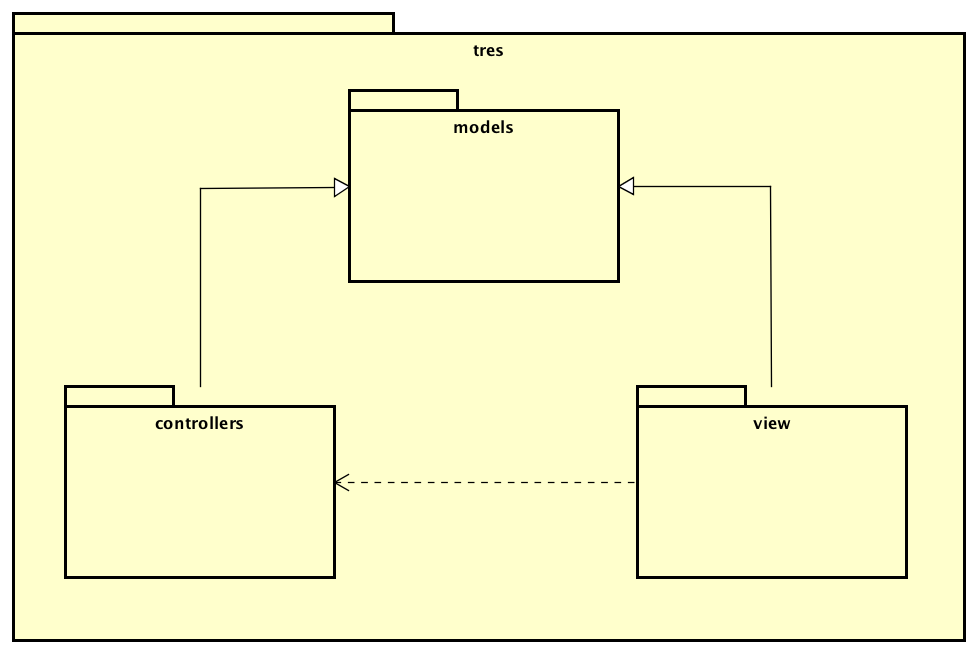
\includegraphics[scale=0.20]{immagini/mvc}
\caption{Contesto di utilizzo del \emph{design pattern \gls{mvc}}}
\label{fig:pattern-mvc}
\end{figure}
\begin{itemize}
\item\textbf{Scopo dell'utilizzo:} questo \emph{design pattern} viene utilizzato per separare i compiti delle diverse componenti \emph{software} dell'applicazione. separa \emph{business logic}, \emph{application logic} e viste, rappresentate rispettivamente da \emph{models}, \emph{controller} e \emph{views};
\item \textbf{Contesto di utilizzo:} questo \emph{pattern} viene implementato nativamente dal \emph{framework} Play. In particolare implementa una tipologia di \emph{\gls{mvc} pull-model}, che permette un salto tecnologico tra la \emph{view} e il \emph{controller}. Questo \emph{pattern} architetturale è importante, perché permette ai programmatori di lavorare sulle componenti di logica applicativa e ai grafici sulle componenti di interfaccia grafica.
\end{itemize}
\subsubsection{\gls{dao}}
\begin{figure}[h]
\centering
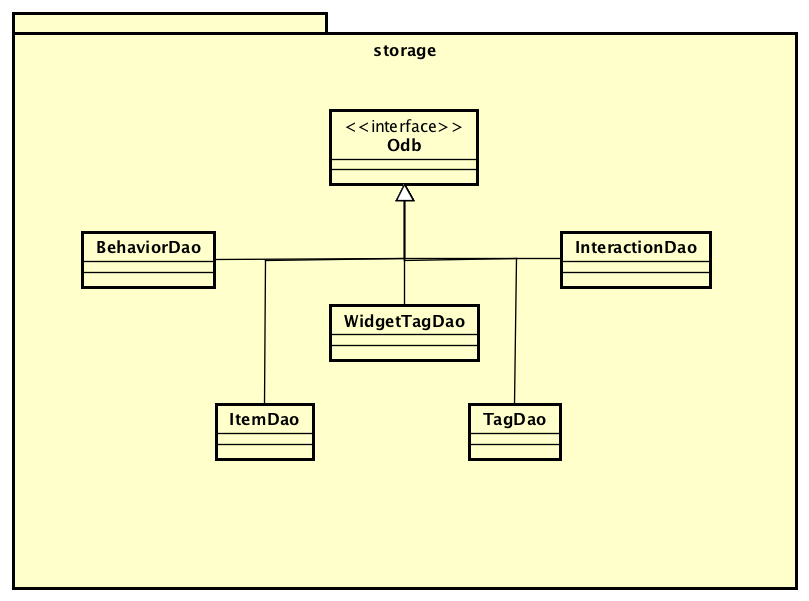
\includegraphics[scale=0.20]{immagini/storage}
\caption{Contesto di utilizzo del \emph{design pattern \gls{dao}}}
\label{fig:pattern-dao}
\end{figure}
\begin{itemize}
\item\textbf{Scopo dell'utilizzo:} questo \emph{design pattern} è utilizzato per disaccoppiare la logica di \emph{business} dalla logica di persistenza. Rende così le componenti indipendenti dal sistema di \emph{database};
\item \textbf{Contesto di utilizzo:} viene utilizzato dalle componenti presenti nel \emph{package storage}, per interagire col \emph{database} OrientDb. L'azienda utilizza diverse tecnologie di persistenza dei dati, quindi per essere facilmente interscambiabile in scenari futuri, è importante l'utilizzo di questo pattern che permette una facile transizione da una tecnologia all'altra.
\end{itemize}
\subsubsection{Strategy}
\begin{figure}[h]
\centering
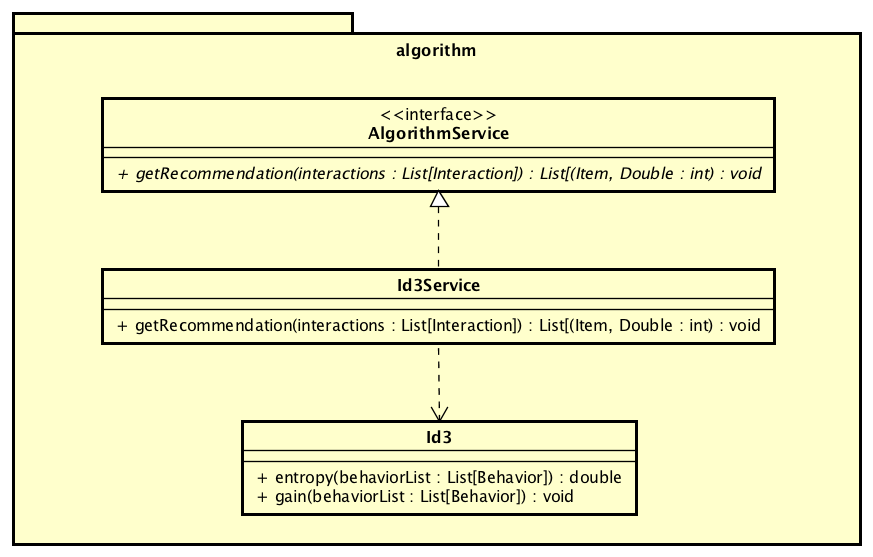
\includegraphics[scale=0.30]{immagini/algorithm}
\caption{Contesto di utilizzo del \emph{design pattern strategy}}
\label{fig:pattern-strategy}
\end{figure}
\begin{itemize}
\item\textbf{Scopo dell'utilizzo:} il \emph{design pattern strategy} definisce una famiglia di algoritmi, incapsulati e resi intercambiabili. \emph{Strategy} permette agli algoritmi di variare indipendentemente dai \emph{client} che ne fanno uso;
\item \textbf{Contesto di utilizzo:} viene utilizzato dalle componenti presenti nel \emph{package algorithm}. E' presente una interfaccia per l'algoritmo. Essa viene implementata da \emph{Id3Service}, che realizza l'algoritmo \emph{ID3}. Ho ritenuto importante applicare questo \emph{pattern} nell'ottica di rendere l'algoritmo facilmente interscambiabile, con altri algoritmi di raccomandazione, come ad esempio degli algoritmi basati sulla teoria dei giochi.
\end{itemize}
\newpage
\subsubsection{Singleton}
\begin{figure}[h]
\centering
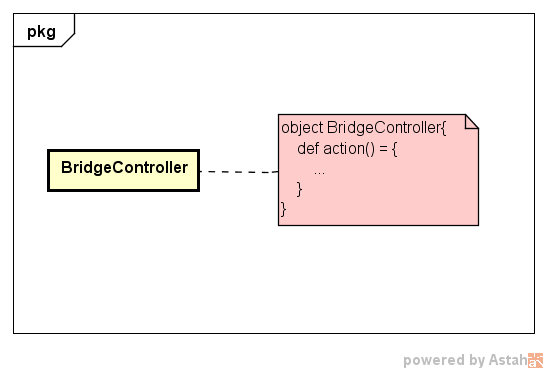
\includegraphics[scale=0.50]{immagini/singleton}
\caption{Contesto di utilizzo del \emph{design pattern singleton}}
\label{fig:pattern-singleton}
\end{figure}
\begin{itemize}
\item\textbf{Scopo dell'utilizzo:} il \emph{design pattern singleton} assicura che una certa classe abbia una sola istanza e fornisce un punto d'acceso globale a tale istanza;
\item \textbf{Contesto di utilizzo:} viene utilizzato nelle componenti del \emph{package controller}. Viene implementato nativamente dal linguaggio Scala dichiarando la classe come \emph{object}. L'utilizzo di questo pattern è fondamentale in questo contesto perché permette il controllo completo delle modalità e tempistiche di accesso del \emph{client}.
\end{itemize}
%**************************************************************



%**************************************************************
\newpage
\section{Progettazione di dettaglio}
La progettazione di dettaglio, con la metodologia \emph{agile}, avviene di pari passo durante la codifica, il che è rischioso perché introduce molti errori di codifica. E' necessario avere una forte conoscenza del dominio tecnico, per poter procedere e non cadere nel modello \emph{code and fix}. Rispetto alle metodologie tradizionali, il focus si sposta nella codifica anziché nella progettazione. Quindi le ore risparmiate della progettazione di dettaglio, sono state reimpiegate nel correggere eventuali errori di codifica. Riporto qui di seguito i diagrammi di sequenza \emph{UML} più significativi:
\subsection{Controllo stato}
In fase di \emph{startup} il sistema non possiede nessun dato, quindi non è in grado di fornire raccomandazioni. Mediante questa chiamata dell'interfaccia \gls{rest}, è possibile verificare lo stato operativo del modulo:\\
\def\arraystretch{1.5}
\begin{longtable}{|p{2.5cm}|p{5cm}|l|}
\hline
\textbf{Tipo} &	\textbf{Chiamata}	\\\hline
GET		&	/tres/ready		 \\\hline
\end{longtable}
\begin{figure}[h]
\centering
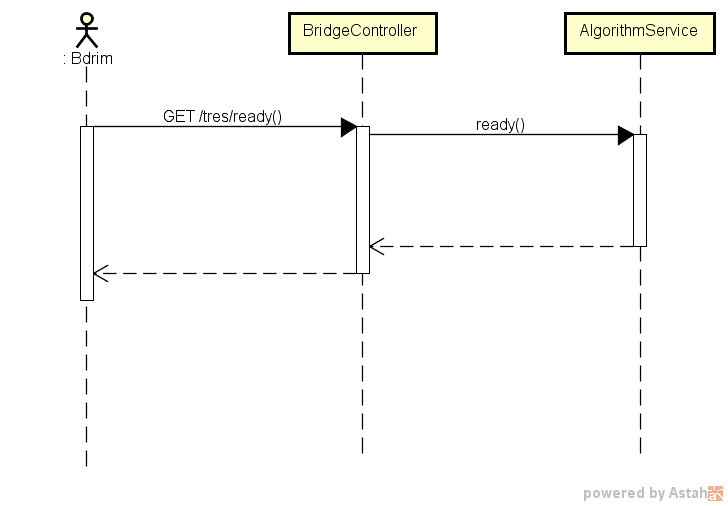
\includegraphics[scale=0.43]{immagini/DScheckstate}
\caption{Diagramma di sequenza: controllo stato.}
\label{fig:seq-controllostato}
\end{figure}
La richiesta \emph{HTTP} giunge fino ad al metodo \emph{ready} della classe \emph{BridgeController}, mediante il \emph{router}. Questo metodo controllerà la presenza dell'albero tramite \emph{AlgorithmService}. Al termine ritorna in \emph{output} una risposta \emph{HTTP}, contenente un oggetto \gls{json}.
\newpage
\subsection{Inserimento behavior}
Per istruire l'algoritmo di selezione, è necessario fornire dei dati per l'apprendimento. Ho implementato una procedura di inserimento dei comportamenti, mediante questa chiamata dell'interfaccia \gls{rest}:
\def\arraystretch{1.5}
\begin{longtable}{|p{2.5cm}|p{5cm}|l|}
\hline
\textbf{Tipo} &	\textbf{Chiamata}	\\\hline
POST	&	/tres/behavior	 \\\hline
\end{longtable}
\begin{figure}[h]
\centering
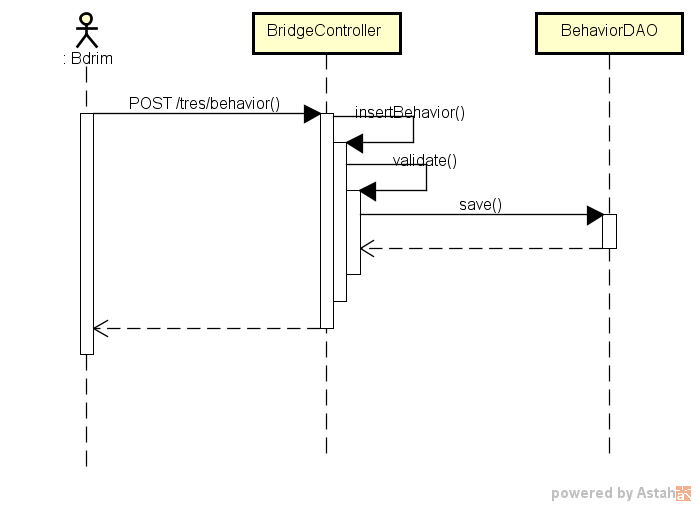
\includegraphics[scale=0.42]{immagini/DSinsertBeh}
\caption{Diagramma di sequenza: inserimento comportamento.}
\label{fig:seq-inserimentobeh}
\end{figure}
Da Bdrim arriva una richiesta \emph{HTTP POST}, che comprende un \gls{json} contenente un \emph{Behavior}. Il \emph{router} di Play accoglie la richiesta, che la reindirizza al metodo della classe \emph{BridgeController insertBehavior}. Il flusso continua con la validazione del \gls{json}. Successivamente il metodo inserisce il comportamento, invocando il metodo \emph{save} della classe \emph{BehaviorDAO}. 


\subsection{Raccomandazione}
Una volta raccolti almeno 100 \emph{Behavior} e che l'algoritmo ha generato l'albero, il sistema è in grado di fornire una raccomandazione. Ho implementato la procedura di raccomandazione, mediante questa chiamata dell'interfaccia \emph{REST}:
\def\arraystretch{1.5}
\begin{longtable}{|p{2.5cm}|p{5cm}|l|}
\hline
\textbf{Tipo} &	\textbf{Chiamata}	\\\hline
POST	&	/tres/recommendation	 \\\hline
\end{longtable}
\begin{figure}[h]
\centering
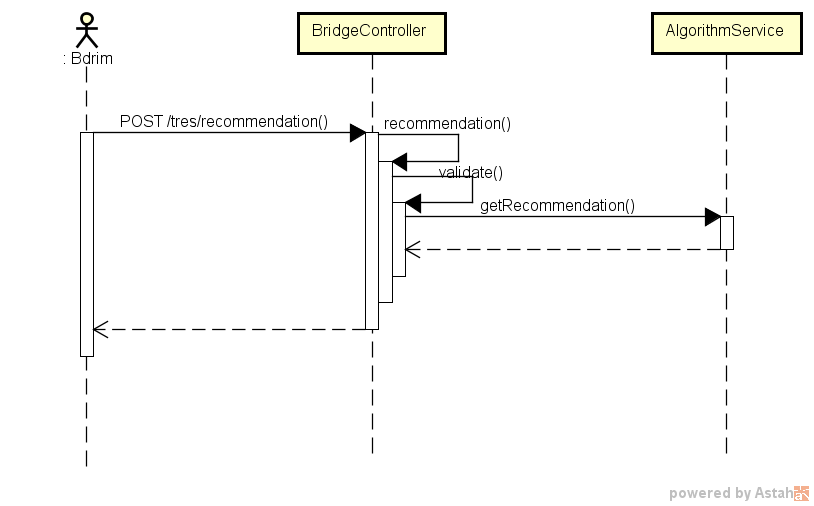
\includegraphics[scale=0.42]{immagini/DSracommandazione}
\caption{Diagramma di sequenza: raccomandazione.}
\label{fig:get-recommendation}
\end{figure}
Da Bdrim arriva una richiesta \emph{HTTP POST}, che comprende un \gls{json} contenente le interazioni dell'utente. Il \emph{router} convoglia la richiesta al metodo \emph{recommendation}, di \emph{BridgeController}. Il flusso procede con la validazione del \gls{json} ricevuto, che estrapola una lista di interazioni dell'utente. Questa lista viene elaborata dall'albero, tramite la chiamata al metodo \emph{getRecommendation} di \emph{AlgorithmService}, che ritornerà le probabilità delle raccomandazioni. 
%**************************************************************




%**************************************************************
\newpage
\section{Verifica e Validazione}%procedere da qui
Questa sezione descrive l'attività di verifica e validazione svolta durante la realizzazione di Tres. Sono elencati gli strumenti utilizzati, le metriche utilizzate e infine un resoconto finale dei test. L'attività di verifica, mi ha permesso di individuare prontamente errori di codifica e ridurre i tempi di sviluppo. Ho cercato di automatizzare il più possibile questa attività, per focalizzarmi nello sviluppo. In primis, ho effettuato dei test di unità per le componenti più complesse. Successivamente ho verificato la loro integrazione. Per motivi di tempo, non ho potuto realizzare tutti i test di unità e di integrazione. Mi sono, quindi, focalizzato sulle componenti principali. 
\subsubsection{Strumenti}
Durante lo sviluppo, ho utilizzato il più possibile degli automatismi. Risparmiando più tempo possibile durante l'analisi statica e dinamica . Ho adottato i seguenti strumenti:
\begin{itemize}
\item \textbf{Intellij IDEA:} questo \gls{ide} fornisce funzionalità per identificare errori di programmazione. Come ad esempio sintassi errata, incompatibilità tra tipi e variabili non definite. Fornisce la percentuale di documentazione dell'intero progetto.
\item \textbf{TravisCI:} è uno strumento che fornisce un automatismo, per la compilazione e l'esecuzione dei \emph{test} del progetto. Se la compilazione o almeno un test fallisce, invia una notifica via \emph{email}, con la possibilità di consultare il \emph{log}.
\item \textbf{Codecov:} questo strumento fornisce la percentuale delle linee di codice coperte durante i \emph{test}.
\item \textbf{Specs2:} è una libreria di \emph{testing}, fornita direttamente da Play Framework. Mi ha permesso di testare l'intera applicazione, anche con le chiamate HTTP.
\end{itemize}
\newpage
\subsubsection{Metriche adottate}
Per la realizzazione di Tres ho adottato le seguenti metriche:
\begin{itemize}
\item \textbf{Attributi per classe:} un numero troppo elevato di attributi, potrebbe indicare la necessità di suddividere la classe in una gerarchia. Ho fissato un \emph{range} ottimale con i seguenti valori: un minimo 1 fino ad un massimo di 8;
\item \textbf{Complessità ciclomatica:} è un indice utilizzato per misurare la complessità di: funzioni, metodi, moduli e classi di un programma. Misura direttamente il numero di cammini linearmente indipendenti, attraverso il grafo di controllo di flusso. I nodi del grafo corrispondono a gruppi indivisibili di istruzioni, mentre gli archi connettono due nodi, se il secondo gruppo di istruzioni può essere eseguito immediatamente dopo il primo gruppo. Per questa metrica ho fissato un \textit{range} ottimale, da un minimo di 1 fino ad un massimo di 10;
\item \textbf{Copertura dei commenti:} è indice della percentuale di classi e metodi corredati di commenti. Ho fissato un range ottimale da 80\% a 100\%;
\item \textbf{Copertura dei test:} è una metrica utilizzata per misurare l'efficacia del collaudo. Si utilizza un indice, che tiene traccia di quante volte è stata eseguita ogni istruzione, durante il \emph{testing}. Le istruzioni eseguite almeno una volta sono dette "coperte". L'obiettivo è coprire il maggior numero possibile di istruzioni. In modo da avere una minore quantità di errore. Per questa metrica ho fissato un valore ottimale minimo di 70\%.
\end{itemize}
\subsection{Resoconto risultati}
\subsubsection{Metriche misurate}
Qui di seguito sono riportate le metriche software misurate:
\begin{itemize}
\item \textbf{Complessità ciclomatica:} per il calcolo della complessità ciclomatica ho utilizzato Sbt, al suo interno è disponibile il \emph{tool} styleCheck. Questo strumento segnala, con un \emph{warning}, se la complessità supera il valore 10. Il \emph{tool} ha restituito esito positivo e non ha segnalato alcun \emph{warning};
\item \textbf{Attributi per classe:} ho rilevato per questa metrica come valore medio 2, mentre come valore massimo ho rilevato 4;
\item \textbf{Copertura commenti:} il valore di copertura è pari al 100\%;
\item \textbf{Copertura dei test:} il valore di copertura dei \emph{test} è del 73\%.
\end{itemize}
\newpage
\subsubsection{Test di unità e di integrazione}
I \emph{test} di unità vengono svolti incrementalmente, durante la codifica di ogni componente. I primi \emph{test} che ho effettuato, riguardano principalmente le componenti base del \emph{models} e quelle responsabili delle iterazioni con il \emph{database}. Successivamente sono passato al \emph{testing} della parte di algoritmica, presente nel \emph{package algorithm}. Per i \emph{test} di unità, ho evitato di utilizzare \emph{mock} e \emph{stub} per le componenti base presenti in \emph{commons}. In quanto ritenevo quelle componenti, molto elementari e che non avrebbero introdotto errori o comportamenti non attesi. Per l'integrazione delle componenti, ho seguito un approccio \emph{bottom-up}. Questo mi ha aiutato a ridurre i tempi di \emph{testing}, evitando sprechi di risorse utilizzando \emph{mock} e {stub}. Ho focalizzato i \emph{test} di integrazione nella parte di algoritmica e in quelle di interazione col \emph{database}. Perché l'incertezza del comportamento di quelle componenti era altissima. Al netto dell'attività di \emph{testing}, i test di unità eseguiti ammontano ad un totale di 10, di cui 10 hanno esito positivo. Per quanto riguarda l'integrazione delle componenti, sono stati eseguiti un totale di 3 \emph{test} di integrazione, di cui 3 hanno avuto esito positivo.

%\subsubsection{Test di unità}
%Qui di seguito sono riportati tutti i \emph{test} di unità eseguiti e il loro relativo esito:
%\def\arraystretch{1.8}
%\begin{longtable}{|l|p{7cm}|l|}
%\hline
%\textbf{Test} &	\textbf{Descrizione}	&	\textbf{Stato}	\\\hline
%TU1	&	Viene verificato che il sistema salvi correttamente un comportamento all'interno del \emph{database}	&	Esito positivo	\\\hline
%TU2	&	Viene verificato il corretto caricamento di una lista di \emph{widgetTag} distinti	&	Esito positivo	\\\hline
%TU3	&	Viene verificato il corretto caricamento di una lista di \emph{item} distinti	&	Esito positivo	\\\hline
%TU4	&	Viene verificato il corretto caricamento di una lista di \emph{behavior} con una \emph{interaction} specifica	&	Esito positivo	\\\hline
%TU5	&	Viene verificato il corretto caricamento di una lista di \emph{behavior} con \emph{tag} e \emph{action} specifici	&	Esito positivo	\\\hline
%TU6	&	Viene verificato il corretto caricamento di una lista di \emph{action} distinti	&	Esito positivo	\\\hline
%TU7	&	Viene verificato il corretto calcolo dell'entropia	&	Esito positivo	\\\hline
%TU8	&	Viene verificato il corretto calcolo del guadagno di informazione	&	Esito positivo	\\\hline
%TU9	&	Viene verificato che venga creata la raccomandazione corretta da fornire	&	Esito positivo	\\\hline
%TU10	&	Viene verificato il corretto calcolo delle probabilità	&	Esito positivo	\\\hline
%\caption{Tabella dei \emph{test} di unità}
%\end{longtable}
%\subsubsection{Test di integrazione}
%Qui di seguito sono riportati tutti i \emph{test} di integrazione eseguiti e il loro relativo esito:
%\def\arraystretch{1.8}
%\begin{longtable}{|l|p{7cm}|l|l|}
%\hline
%\textbf{Test} &	\textbf{Descrizione}	&	\textbf{Componente}	&	\textbf{Stato}	\\\hline
%TI1	&	Viene verificato che il sistema crei correttamente un albero di decisione	&	algorithm	&	Esito positivo	\\\hline
%TI2	&	Viene verificato che il sistema aggiorni l'albero di decisione ogni 24 ore	&	algorithm	&	Esito positivo	\\\hline
%TI3	&	Viene verificata la corretta creazione del \emph{training set}		&	algorithm	&	Esito positivo	\\\hline
%\caption{Tabella dei \emph{test} di integrazione}
%\end{longtable}
\subsubsection{Test di sistema}
Ho effettuato alcuni \emph{test} di sistema inerenti alle funzionalità di: inserimento dati, calcolo di una raccomandazione e infine calcolo probabilità.
\begin{itemize}
\item \textbf{Inserimento dati:} viene verificato il corretto comportamento del sistema alla richiesta di inserimento dati;
\item \textbf{Calcolo raccomandazioni:} viene verificato il calcolo della raccomandazione da fornire;
\item \textbf{Calcolo probabilità:} viene verificato il calcolo delle probabilità associate ai vari \emph{item}.
\end{itemize}
%***************************************************************************************************************




%***************************************************************************************************************
\newpage
\section{Sommario funzionamento}
Questa sezione descrive il funzionamento del sistema realizzato durante lo stage. Qui di seguito viene illustrato il funzionamento dal punto di vista del \emph{client} che utilizza il modulo.
\begin{figure}[h]
\centering
\includegraphics[scale=0.42]{immagini/flux}
\caption{Diagramma di sequenza: raccomandazione.}
\label{fig:flux}
\end{figure}
\newpage
In fase di \emph{startup} il sistema non possiede nessun dato. Esso quindi non è in grado di fornire raccomandazioni. Il \emph{client} deve dunque verificare lo stato di operatività del sistema, attraverso una chiamata \emph{HTTP} a:\\
\begin{center}
GET    /tres/ready
\end{center}
Il client ottiene così un oggetto \gls{json} simile al seguente.
\begin{lstlisting}[language=json,firstnumber=1]
{
  "ready":false
}
\end{lstlisting}
La risposta \emph{HTTP} ritorna un oggetto \gls{json} contenente un \emph{booleano}, che indica l'operatività del modulo. L'operatività dipende essenzialmente dal numero di comportamenti utente inseriti nel sistema. Se il modulo non è operativo, si continua con la procedura di inserimento dei comportamenti tramite la chiamata:
\begin{center}
POST    /tres/behavior
\end{center}
L'oggetto da inviare tramite questa chiamata deve contenere un \gls{json} simile al seguente.
\begin{lstlisting}[language=json,firstnumber=1]
{
  "item":{
    "tags":[
      {
        "name":"tag:uno"
      },
      {
        "name":"tag:due"
      }
    ]
  },
  "interactions":[
    {
      "widgetTag":{
        "name":"Income"
      },
      "action":"High"
    },
    {
      "widgetTag":{
        "name":"PreviousCustomer"
      },
      "action":"No"
    }
  ]
}
\end{lstlisting}
Un comportamento si registra solamente quando le azioni dell'utente hanno prodotto un risultato all'interno del sito (come ad esempio un acquisto nel caso di un \emph{e-commerce}). Una volta generato l'albero, Tres è in grado di fornire raccomandazioni agli utenti. Il \emph{client}, quindi, può iniziare la procedura per richiedere una raccomandazione. Esso, innanzitutto, deve richiedere a Tres quale argomento con cui interrogare l'utente. Mediante la seguente chiamata \emph{HTTP} è possibile richiedere l'argomento: 
\begin{center}
POST    /tres/answer
\end{center}
\newpage
La chiamata deve comprendere un oggetto \gls{json}, che contiene le interazioni che l'utente ha già svolto.
\begin{lstlisting}[language=json,firstnumber=1]
{
  "interactions":[
    {
      "widgetTag":{
        "name":"District"
      },
      "action":"Urban"
    },
    {
      "widgetTag":{
        "name":"HouseType"
      },
      "action":"Semi-Detached"
    }  
  ]
}
\end{lstlisting}
Questa chiamata fornisce come risposta il prossimo \emph{WidgetTag} da utilizzare, per interrogare l'utente del sito come il seguente oggetto \gls{json}.
\begin{lstlisting}[language=json,firstnumber=1]
{
  name: "Income"
}
\end{lstlisting}
L'utente va ad interagire con il \emph{WidgetTag} con cui lo interroghiamo. Dopodiché il \emph{client} aggiunge l'interazione alle interazioni precedentemente salvate. Il \emph{client} deve continuare a reiterare questa chiamata, aggiungendo le interazioni. Finché Tres continua a fornire dei \emph{WidgetTag}, per interrogare l'utente. Se Tres non ne fornisce altri, significa che la classificazione del comportamento è terminata. E' quindi possibile per il \emph{client}, procedere con la richiesta della raccomandazione. La chiamata \emph{HTTP} da effettuare è la seguente:
\begin{center}
POST    /tres/recommendation
\end{center}
Nella chiamata dev'essere presente il \gls{json} contenente le interazioni dell'utente. La risposta di Tres comprende un oggetto \gls{json}, dove vengono indicate le percentuali dei prodotti/oggetti/post da raccomandare all'utente.
\begin{lstlisting}[language=json,firstnumber=1]
{
  "items":[
    {
      "item":{
        "tags":[
          {
            "name":"tag:uno"
          },
          {
            "name":"tag:due"
          }
        ]
      },
      "percentage":100
    }
  ]
}
\end{lstlisting}
Quando il comportamento dell'utente ha prodotto un risultato, il \emph{client} inserisce il suo comportamento nel sistema e termina la procedura.
%**************************************************************
             % Il progetto di stage
% !TEX encoding = UTF-8
% !TEX TS-program = pdflatex
% !TEX root = ../tesi.tex
% !TEX spellcheck = it-IT

%**************************************************************
\chapter{Valutazione Retrospettiva}
\label{cap:valutazione-retrospettiva}
%**************************************************************
\intro{Questo capitolo riporta un bilancio finale su quanto svolto durante lo stage.}




%**************************************************************************************************
\section{Bilancio sui risultati}
In questa sezione riassumo gli obiettivi aziendali e gli obiettivi personali raggiunti durante lo stage.
\subsection{Obiettivi conseguiti}
Gli obiettivi fissati all'inizio dello stage, hanno subito delle modifiche. L'azienda ha voluto privilegiare il \emph{porting} di DRE. Il \emph{porting} dell'applicativo è parzialmente completato. L'unica funzionalità non ancora implementata è una procedura di \emph{map-reduce}. Questa funzionalità non l'ho completata, perché le mie competenze per comprendere quel codice erano insufficienti. Le parti su cui intervenire erano scritte in javascript, sistemarle avrebbe introdotto un ulteriore ritardo per lo sviluppo di Tres. L'obiettivo di migliorare la fase di apprendimento di questo modulo non l'ho raggiunto. Durante lo sviluppo di Tres ho individuato 23 requisiti, di cui, come raffigurato in \ref{fig:graficorequisiti}, 20 obbligatori e 3 desiderabili.  
\begin{figure}[h]
\centering
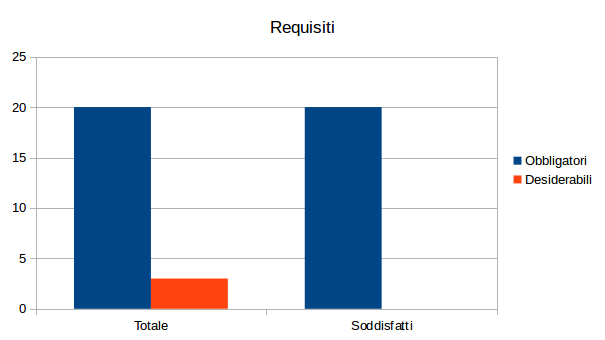
\includegraphics[scale=0.64]{immagini/graficorequisiti}
\caption{Riassunto requisiti}
\label{fig:graficorequisiti}
\end{figure}
\\I requisiti desiderabili non soddisfatti riguardavano l'implementazione di algoritmi di \emph{clustering}, pertanto questo scopo non è stato raggiunto.
Tuttavia ho raggiunto l'obiettivo di implementare algoritmi per l'individuazione dei gusti dell'utente, grazie all'implementazione di \emph{ID3}. In questo stage ho conseguito il \emph{target} minimo riguardante l'utilizzo di OrientDb. Durante le due attività di porting e sviluppo, ho avuto modo di utilizzare questa tecnologia. 
\subsection{Obiettivi personali}
All'inizio dello stage, il mio scopo era di imparare nuove tecnologie da aggiungere alle mie conoscenze. Ritenevo il mio bagaglio professionale insufficiente, per affrontare il mondo del lavoro. Lo stage mi ha permesso di padroneggiare molte tecnologie, quali: OrientDb, Scala e un \emph{web \gls{framework}} di concezione moderna. Scala mi ha dato la possibilità di apprendere le nozioni per un corretto stile di programmazione funzionale. Mi ero prefissato di approfondire argomenti quali, intelligenza artificiale e i sistemi di raccomandazione. Ritengo questo parzialmente soddisfatto. Non ho trovato il supporto necessario per approfondire queste competenze, soprattutto per i sistemi di raccomandazione.
%**************************************************************************************************




%**************************************************************************************************
\section{Bilancio formativo}
In questa sezione riporto le competenze acquisite durante lo stage.\\
Lo stage in Nextep Srl è stata la  mia prima esperienza nel settore informatico. Mi ha permesso di apprendere nuove competenze e consolidare competenze già apprese durante il corso di studi.
%Prima avevo idee molto confuse a riguardo la mia carriera professionale, ma ora dopo lo stage posso affermare di avere aspettative più ambiziose e idee più chiare su quale cammino professionale intraprendere.
Ho trovato molto positivo lavorare collaborativamente al progetto, perché questo mi ha portato a migliorare le mie capacità di \emph{team working}. Questa abilità è molto importante nel mondo del lavoro, soprattutto nei contesti lavorativi dove si utilizza una metodologia \emph{agile}. Ho migliorato le mie capacità di \emph{project management} per concludere il progetto nei tempi fissati e raggiungere gli obbiettivi minimi che mi sono prefissato. In conclusione, ho terminato lo stage con un bagaglio professionale più ricco e di essere in grado di farmi carico di responsabilità più importanti.
\newpage
\subsubsection{Scala}
Durante lo stage ho avuto modo di apprezzare i vantaggi derivanti dall'uso di questo linguaggio. Ho utilizzato questa tecnologia nelle attività di \emph{porting} del modulo DRE e nell'attività di sviluppo di Tres. Per studiare Scala ho seguito un corso \emph{online}\footcite{https://www.coursera.org/course/progfun} tenuto direttamente dal professore Martin Odersky\footcite{http://lampwww.epfl.ch/~odersky/}, ovvero il \emph{designer} del linguaggio stesso. Un corso validissimo per capire i meccanismi e le peculiarità di questo linguaggio. All'inizio è stato un po' ostico mettere in pratica quanto appreso, ma quando ho cominciato a padroneggiare Scala ho potuto constatare un aumento della mia produttività. Ho trovato un po' macchinoso gestire la compatibilità con librerie Java di terze parti. Mi ritengo soddisfatto di aver imparato questa tecnologia e di poter reinvestire nel mondo del lavoro questa conoscenza. 
Scala mi ha introdotto al paradigma di programmazione funzionale. Questo paradigma mi ha fornito una modalità diversa di affrontare e risolvere problemi, rispetto alla classica programmazione orientata agli oggetti. Nella programmazione funzionale vengono evitati i dati di stato e modificabili, mentre viene data invece una maggiore enfasi all'applicazione di funzioni. Mantenere gli stati immutabili facilita la suddivisone del codice per l'esecuzione parallela, garantendone la correttezza. Questa caratteristica è importantissima al giorno d'oggi, dove il focus si sta via via spostando sempre di più verso contesti multi-threading. %Per concludere questo paradigma induce ad uno stile di programmazione più espressivo e conciso 
\subsubsection{OrientDb}
Questa tecnologia è la soluzione di persistenza adottata durante il progetto. La curva di apprendimento è stata molto rapida, grazie al corso online\footcite{https://www.udemy.com/orientdb-getting-started/}, tenuto durante l'attività di formazione. Mi ha permesso di imparare le differenze tra i modelli più tradizionali, come i relazionali e i modelli a grafo. I modelli a grafo si prestano molto bene per soluzioni nel dominio web, soprattutto in questo momento storico, dove il web si sta evolvendo in web semantico. E' stato un po' difficoltoso all'inizio passare dal concetto di \emph{Join} delle tabelle al concetto di \emph{Traverse} dei grafi. Tuttavia la modellazione del dominio con un grafo, è stata molto più semplice ed intuitiva rispetto ad un modello relazionale. 
\subsubsection{Play Framework}
L'apprendimento di questo \emph{framework} non è particolarmente difficile. La documentazione presente nel sito è molto esaustiva, fornisce un supporto completo per la configurazione di una web application. Trovo molto vantaggioso la compatibilità con i linguaggi Java e Scala, in modo da poter sviluppare una applicazione con entrambi i linguaggi. La prima configurazione iniziale è stata molto semplice, questo mi ha permesso di focalizzarmi subito nello sviluppo del modulo. Purtroppo ho trovato complicato testare parti del mio modulo, perché  era necessario, per il test, avere l'istanza del server avviata.
%**************************************************************************************************




%**************************************************************************************************
\newpage
\section{Distanza tra formazione universitaria e lavoro}
In questa sezione espongo la valutazione personale, della distanza tra la formazione ricevuta durante il corso di studi e lo stage formativo. 
%Questa esperienza mi ha permesso di valutare la distanza tra la formazione universitaria e le competenze realmente richiesta durante lo stage.
L'insegnamento che mi ha maggiormente preparato ad affrontare lo stage, è sicuramente \emph{Ingegneria del Software}.
Le competenze mancanti ad inizio stage non sono state molte.
Il \emph{gap} formativo è stato adeguato per essere colmato durante le attività svolte. Soprattutto durante l'attività di studio della prima settimana, che mi ha permesso di apprendere le conoscenze necessarie per affrontare le attività successive.\\
L'attività di modellazione del \emph{database} è stata una delle difficoltà maggiori incontrata durante il percorso. La modellazione di una base di dati a grafo, richiede un approccio differente al problema rispetto alle soluzioni relazionali.\\
Una difficoltà minore riguarda la programmazione funzionale. Questo paradigma all'inizio mi è risultato difficoltoso da assimilare, perché abituato ai linguaggi orientati agli oggetti.\\
Uno strumento che ho spesso utilizzato e che non è stato introdotto durante il corso di studi, è il debugger. Questo strumento risulta molto utile, per individuare errori e comportamenti non attesi del codice.\\
Durante lo stage, mi sono mancate le nozioni base per implementare fedelmente una architettura \gls{rest}. Questa tecnologia l'ho già affrontata, durante il progetto finale di ingegneria del software. Ma non è stato sufficiente per assimilarne la filosofia di base.\\
Per concludere le mie lacune più evidenti, sono fondamenti di intelligenza artificiale e i sistemi di raccomandazione. Avere queste nozioni all'inizio dello stage, mi avrebbe sicuramente aiutato durante analisi dei requisiti per il modulo Tres. L'attività di analisi, infatti, è stata in assoluto la difficoltà maggiore. Conoscere il dominio, mi avrebbe permesso di intercettare con più efficacia le esigenze del proponente.
%GIA PREVISTO testing del codice più efficace -> questa abilità è qualificante
%GIA PREVISTO capacità di progettare una architettura flessibile, --> poca enfasi nei design pattern
%GIA PREVISTO NEL CORSO team working -> prevedere più progetti di gruppo
%GIA PREVISTO abilità nel porting dell'applicativo -> introdurre delle best practice


%Per concludere, programmazione asincrona
% fare discorso su debugger????
%L'insegnamento che mi ha maggiormente preparato per questa esperienza, è sicuramente \emph{Ingegneria Del Software}. Grazie a questo corso ho appreso molte nozioni tecniche e un approccio valido per la gestione e la produzione software, un bagaglio molto importante per il mondo del lavoro.
%La prima difficoltà che ho incontrato riguarda l'attività di modellazione del \emph{database}. Mi sarebbe stato utile avere delle nozioni per affrontare una modellazione su di un database a grafo. Durante il corso di \emph{Basi di Dati}, invece, vengono insegnate solamente soluzioni come i \emph{database} relazionali. Sarebbe sufficiente introdurre dei fondamenti sulle varie tipologie di database, in modo che lo studente possa valutare pro e contro di ogni tipologia e utilizzare la soluzione migliore a seconda del contesto.
%Sarebbe utile fornire dei concetti di programmazione funzionale, questo stile di programmazione risulta molto adatto per soluzioni \emph{multi-threading}. Si potrebbe introdurre questi concetti durante il corso di \emph{programmazione concorrente e distribuita}, sempre col medium di Java, in modo sfruttare facilmente il parallelismo offerto dalle odierne architetture.
%A livello tecnico, ritengo che durante il corso di laurea sia dato poco spazio per apprendere e consolidare tecniche di programmazione valide, ed evitare quindi errori comuni in sede lavorativa. Dovrebbero essere introdotti i design pattern e il loro corretto utilizzo durante il corso di \emph{programmazione ad oggetti}.
%Sarebbe importante, nel corso di \emph{Programmazione}, spiegare come utilizzare strumenti per fare \emph{debug} del codice. Padroneggiare questo strumento risulta molto utile soprattutto in ambito lavorativo.
%Concludo affermando che il corso di laurea, mi ha fornito le nozioni fondamentali per poter affrontare egregiamente il mondo del lavoro.
%**************************************************************************************************
             % Valutazioni retrospettive
\appendix                               
%% !TEX encoding = UTF-8
% !TEX TS-program = pdflatex
% !TEX root = ../tesi.tex
% !TEX spellcheck = it-IT

%**************************************************************
\chapter{Appendice A}
%**************************************************************

\epigraph{Citazione}{Autore della citazione}



             % Appendice A

%**************************************************************
% Materiale finale
%**************************************************************
\backmatter
\printglossaries
% !TEX encoding = UTF-8
% !TEX TS-program = pdflatex
% !TEX root = ../tesi.tex
% !TEX spellcheck = it-IT

%**************************************************************
% Bibliografia
%**************************************************************

\cleardoublepage
\chapter{Bibliografia}

\nocite{*}
%\printbibliography

\bibbycategory % equivale a dare un \printbibliography per ogni categoria


\end{document}\grid
